\begin{minipage}[b]{0.15\linewidth}
\begin{figure}[H]                                                          
  \centering                                                             
  \begin{adjustbox}{width=1.5cm,center}                                   
  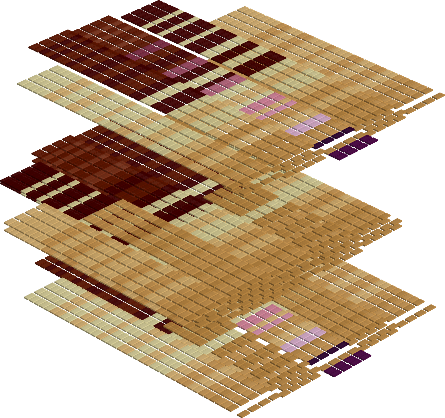
\includegraphics[width=1.5cm]{src/colorspace_colourflow/flows/colourflow_42-45.png}%           
  \end{adjustbox}                                                        
\caption*{

\begin{tikzpicture}                             
\definecolor{tempcolor}{HTML}{000000}           
\fill[tempcolor] (1 mm,0) rectangle ++(1mm,1mm);
\definecolor{tempcolor}{HTML}{db9f4e}           
\fill[tempcolor] (2 mm,0) rectangle ++(1mm,1mm);
\definecolor{tempcolor}{HTML}{ecb05f}           
\fill[tempcolor] (3 mm,0) rectangle ++(1mm,1mm);
\definecolor{tempcolor}{HTML}{ffd285}           
\fill[tempcolor] (4 mm,0) rectangle ++(1mm,1mm);
\definecolor{tempcolor}{HTML}{fff4b2}           
\fill[tempcolor] (5 mm,0) rectangle ++(1mm,1mm);
\definecolor{tempcolor}{HTML}{4f0000}           
\fill[tempcolor] (6 mm,0) rectangle ++(1mm,1mm);
\definecolor{tempcolor}{HTML}{711900}           
\fill[tempcolor] (7 mm,0) rectangle ++(1mm,1mm);
\definecolor{tempcolor}{HTML}{933b1e}           
\fill[tempcolor] (8 mm,0) rectangle ++(1mm,1mm);
\end{tikzpicture}                               
}
\end{figure}                                                               
\end{minipage}
\hspace{0.1cm}
\begin{minipage}[b]{0.15\linewidth}
\begin{figure}[H]                                                          
  \centering                                                             
  \begin{adjustbox}{width=1.5cm,center}                                   
  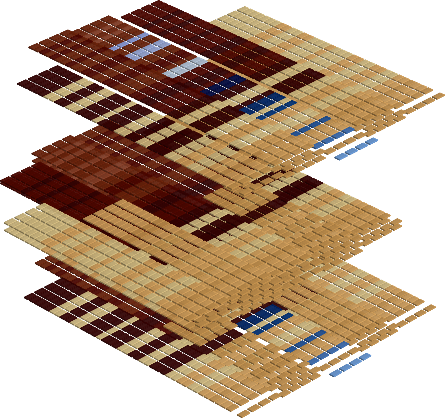
\includegraphics[width=1.5cm]{src/colorspace_colourflow/flows/colourflow_43-45.png}%           
  \end{adjustbox}                                                        
\caption*{

\begin{tikzpicture}                             
\definecolor{tempcolor}{HTML}{000000}           
\fill[tempcolor] (1 mm,0) rectangle ++(1mm,1mm);
\definecolor{tempcolor}{HTML}{ecb05f}           
\fill[tempcolor] (2 mm,0) rectangle ++(1mm,1mm);
\definecolor{tempcolor}{HTML}{fdc170}           
\fill[tempcolor] (3 mm,0) rectangle ++(1mm,1mm);
\definecolor{tempcolor}{HTML}{ffe39c}           
\fill[tempcolor] (4 mm,0) rectangle ++(1mm,1mm);
\definecolor{tempcolor}{HTML}{420404}           
\fill[tempcolor] (5 mm,0) rectangle ++(1mm,1mm);
\definecolor{tempcolor}{HTML}{600800}           
\fill[tempcolor] (6 mm,0) rectangle ++(1mm,1mm);
\definecolor{tempcolor}{HTML}{822a0d}           
\fill[tempcolor] (7 mm,0) rectangle ++(1mm,1mm);
\definecolor{tempcolor}{HTML}{a44c2f}           
\fill[tempcolor] (8 mm,0) rectangle ++(1mm,1mm);
\end{tikzpicture}                               
}
\end{figure}                                                               
\end{minipage}
\hspace{0.1cm}
\begin{minipage}[b]{0.15\linewidth}
\begin{figure}[H]                                                          
  \centering                                                             
  \begin{adjustbox}{width=1.5cm,center}                                   
  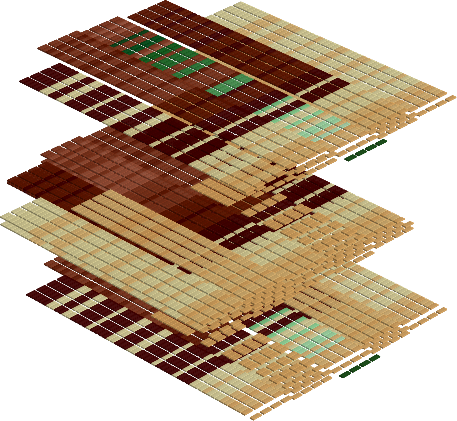
\includegraphics[width=1.5cm]{src/colorspace_colourflow/flows/colourflow_44-45.png}%           
  \end{adjustbox}                                                        
\caption*{

\begin{tikzpicture}                             
\definecolor{tempcolor}{HTML}{000000}           
\fill[tempcolor] (1 mm,0) rectangle ++(1mm,1mm);
\definecolor{tempcolor}{HTML}{fdc170}           
\fill[tempcolor] (2 mm,0) rectangle ++(1mm,1mm);
\definecolor{tempcolor}{HTML}{ffd285}           
\fill[tempcolor] (3 mm,0) rectangle ++(1mm,1mm);
\definecolor{tempcolor}{HTML}{fff4b2}           
\fill[tempcolor] (4 mm,0) rectangle ++(1mm,1mm);
\definecolor{tempcolor}{HTML}{4f0000}           
\fill[tempcolor] (5 mm,0) rectangle ++(1mm,1mm);
\definecolor{tempcolor}{HTML}{711900}           
\fill[tempcolor] (6 mm,0) rectangle ++(1mm,1mm);
\definecolor{tempcolor}{HTML}{933b1e}           
\fill[tempcolor] (7 mm,0) rectangle ++(1mm,1mm);
\definecolor{tempcolor}{HTML}{b55d40}           
\fill[tempcolor] (8 mm,0) rectangle ++(1mm,1mm);
\end{tikzpicture}                               
}
\end{figure}                                                               
\end{minipage}
\hspace{0.1cm}
\begin{minipage}[b]{0.15\linewidth}
\begin{figure}[H]                                                          
  \centering                                                             
  \begin{adjustbox}{width=1.5cm,center}                                   
  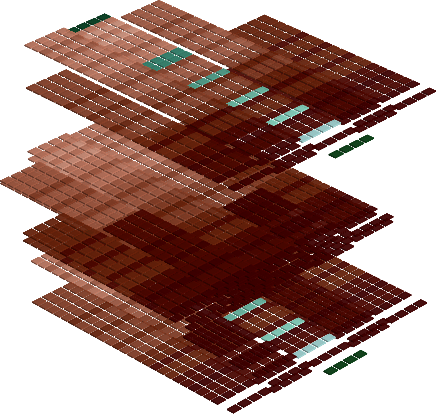
\includegraphics[width=1.5cm]{src/colorspace_colourflow/flows/colourflow_49-45.png}%           
  \end{adjustbox}                                                        
\caption*{

\begin{tikzpicture}                             
\definecolor{tempcolor}{HTML}{000000}           
\fill[tempcolor] (1 mm,0) rectangle ++(1mm,1mm);
\definecolor{tempcolor}{HTML}{4f0000}           
\fill[tempcolor] (2 mm,0) rectangle ++(1mm,1mm);
\definecolor{tempcolor}{HTML}{600800}           
\fill[tempcolor] (3 mm,0) rectangle ++(1mm,1mm);
\definecolor{tempcolor}{HTML}{822a0d}           
\fill[tempcolor] (4 mm,0) rectangle ++(1mm,1mm);
\definecolor{tempcolor}{HTML}{a44c2f}           
\fill[tempcolor] (5 mm,0) rectangle ++(1mm,1mm);
\definecolor{tempcolor}{HTML}{c66e51}           
\fill[tempcolor] (6 mm,0) rectangle ++(1mm,1mm);
\definecolor{tempcolor}{HTML}{e89073}           
\fill[tempcolor] (7 mm,0) rectangle ++(1mm,1mm);
\definecolor{tempcolor}{HTML}{ffb298}           
\fill[tempcolor] (8 mm,0) rectangle ++(1mm,1mm);
\end{tikzpicture}                               
}
\end{figure}                                                               
\end{minipage}
\hspace{0.1cm}
\begin{minipage}[b]{0.15\linewidth}
\begin{figure}[H]                                                          
  \centering                                                             
  \begin{adjustbox}{width=1.5cm,center}                                   
  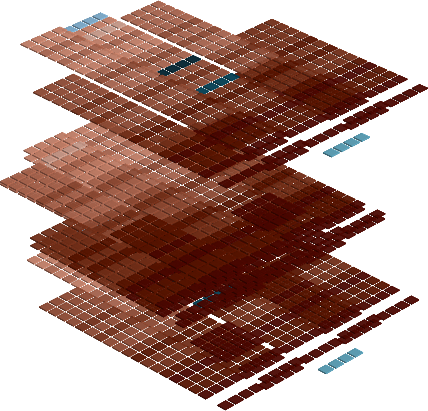
\includegraphics[width=1.5cm]{src/colorspace_colourflow/flows/colourflow_50-45.png}%           
  \end{adjustbox}                                                        
\caption*{

\begin{tikzpicture}                             
\definecolor{tempcolor}{HTML}{000000}           
\fill[tempcolor] (1 mm,0) rectangle ++(1mm,1mm);
\definecolor{tempcolor}{HTML}{600800}           
\fill[tempcolor] (2 mm,0) rectangle ++(1mm,1mm);
\definecolor{tempcolor}{HTML}{711900}           
\fill[tempcolor] (3 mm,0) rectangle ++(1mm,1mm);
\definecolor{tempcolor}{HTML}{933b1e}           
\fill[tempcolor] (4 mm,0) rectangle ++(1mm,1mm);
\definecolor{tempcolor}{HTML}{b55d40}           
\fill[tempcolor] (5 mm,0) rectangle ++(1mm,1mm);
\definecolor{tempcolor}{HTML}{d77f62}           
\fill[tempcolor] (6 mm,0) rectangle ++(1mm,1mm);
\definecolor{tempcolor}{HTML}{f9a183}           
\fill[tempcolor] (7 mm,0) rectangle ++(1mm,1mm);
\definecolor{tempcolor}{HTML}{ffc3ae}           
\fill[tempcolor] (8 mm,0) rectangle ++(1mm,1mm);
\end{tikzpicture}                               
}
\end{figure}                                                               
\end{minipage}
\hspace{0.1cm}
\begin{minipage}[b]{0.15\linewidth}
\begin{figure}[H]                                                          
  \centering                                                             
  \begin{adjustbox}{width=1.5cm,center}                                   
  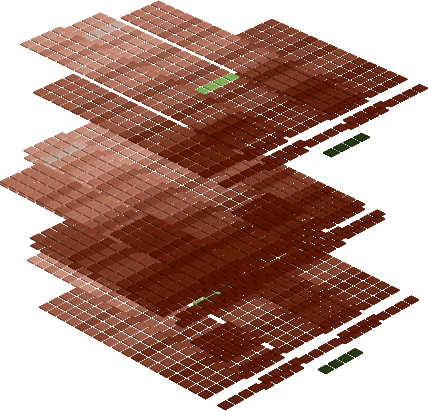
\includegraphics[width=1.5cm]{src/colorspace_colourflow/flows/colourflow_51-45.png}%           
  \end{adjustbox}                                                        
\caption*{

\begin{tikzpicture}                             
\definecolor{tempcolor}{HTML}{000000}           
\fill[tempcolor] (1 mm,0) rectangle ++(1mm,1mm);
\definecolor{tempcolor}{HTML}{711900}           
\fill[tempcolor] (2 mm,0) rectangle ++(1mm,1mm);
\definecolor{tempcolor}{HTML}{822a0d}           
\fill[tempcolor] (3 mm,0) rectangle ++(1mm,1mm);
\definecolor{tempcolor}{HTML}{a44c2f}           
\fill[tempcolor] (4 mm,0) rectangle ++(1mm,1mm);
\definecolor{tempcolor}{HTML}{c66e51}           
\fill[tempcolor] (5 mm,0) rectangle ++(1mm,1mm);
\definecolor{tempcolor}{HTML}{e89073}           
\fill[tempcolor] (6 mm,0) rectangle ++(1mm,1mm);
\definecolor{tempcolor}{HTML}{ffb298}           
\fill[tempcolor] (7 mm,0) rectangle ++(1mm,1mm);
\definecolor{tempcolor}{HTML}{ffd4c4}           
\fill[tempcolor] (8 mm,0) rectangle ++(1mm,1mm);
\end{tikzpicture}                               
}
\end{figure}                                                               
\end{minipage}
\hspace{0.1cm}
\begin{minipage}[b]{0.15\linewidth}
\begin{figure}[H]                                                          
  \centering                                                             
  \begin{adjustbox}{width=1.5cm,center}                                   
  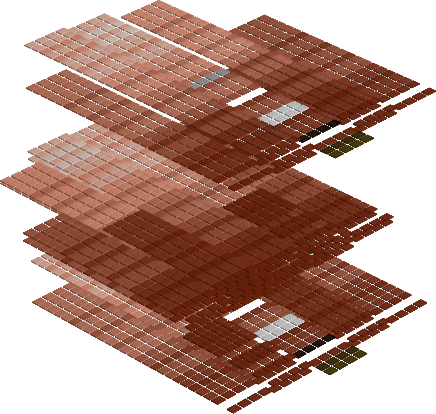
\includegraphics[width=1.5cm]{src/colorspace_colourflow/flows/colourflow_52-45.png}%           
  \end{adjustbox}                                                        
\caption*{

\begin{tikzpicture}                             
\definecolor{tempcolor}{HTML}{000000}           
\fill[tempcolor] (1 mm,0) rectangle ++(1mm,1mm);
\definecolor{tempcolor}{HTML}{822a0d}           
\fill[tempcolor] (2 mm,0) rectangle ++(1mm,1mm);
\definecolor{tempcolor}{HTML}{933b1e}           
\fill[tempcolor] (3 mm,0) rectangle ++(1mm,1mm);
\definecolor{tempcolor}{HTML}{b55d40}           
\fill[tempcolor] (4 mm,0) rectangle ++(1mm,1mm);
\definecolor{tempcolor}{HTML}{d77f62}           
\fill[tempcolor] (5 mm,0) rectangle ++(1mm,1mm);
\definecolor{tempcolor}{HTML}{f9a183}           
\fill[tempcolor] (6 mm,0) rectangle ++(1mm,1mm);
\definecolor{tempcolor}{HTML}{ffc3ae}           
\fill[tempcolor] (7 mm,0) rectangle ++(1mm,1mm);
\definecolor{tempcolor}{HTML}{ffe5da}           
\fill[tempcolor] (8 mm,0) rectangle ++(1mm,1mm);
\end{tikzpicture}                               
}
\end{figure}                                                               
\end{minipage}
\hspace{0.1cm}
\begin{minipage}[b]{0.15\linewidth}
\begin{figure}[H]                                                          
  \centering                                                             
  \begin{adjustbox}{width=1.5cm,center}                                   
  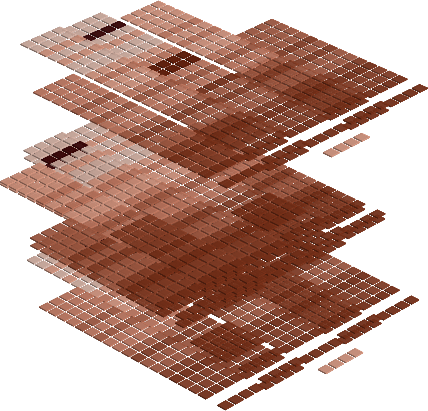
\includegraphics[width=1.5cm]{src/colorspace_colourflow/flows/colourflow_53-45.png}%           
  \end{adjustbox}                                                        
\caption*{

\begin{tikzpicture}                             
\definecolor{tempcolor}{HTML}{000000}           
\fill[tempcolor] (1 mm,0) rectangle ++(1mm,1mm);
\definecolor{tempcolor}{HTML}{933b1e}           
\fill[tempcolor] (2 mm,0) rectangle ++(1mm,1mm);
\definecolor{tempcolor}{HTML}{a44c2f}           
\fill[tempcolor] (3 mm,0) rectangle ++(1mm,1mm);
\definecolor{tempcolor}{HTML}{c66e51}           
\fill[tempcolor] (4 mm,0) rectangle ++(1mm,1mm);
\definecolor{tempcolor}{HTML}{e89073}           
\fill[tempcolor] (5 mm,0) rectangle ++(1mm,1mm);
\definecolor{tempcolor}{HTML}{ffb298}           
\fill[tempcolor] (6 mm,0) rectangle ++(1mm,1mm);
\definecolor{tempcolor}{HTML}{ffd4c4}           
\fill[tempcolor] (7 mm,0) rectangle ++(1mm,1mm);
\definecolor{tempcolor}{HTML}{410103}           
\fill[tempcolor] (8 mm,0) rectangle ++(1mm,1mm);
\end{tikzpicture}                               
}
\end{figure}                                                               
\end{minipage}
\hspace{0.1cm}
\begin{minipage}[b]{0.15\linewidth}
\begin{figure}[H]                                                          
  \centering                                                             
  \begin{adjustbox}{width=1.5cm,center}                                   
  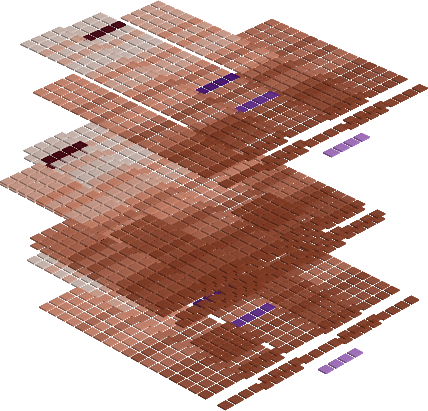
\includegraphics[width=1.5cm]{src/colorspace_colourflow/flows/colourflow_54-45.png}%           
  \end{adjustbox}                                                        
\caption*{

\begin{tikzpicture}                             
\definecolor{tempcolor}{HTML}{000000}           
\fill[tempcolor] (1 mm,0) rectangle ++(1mm,1mm);
\definecolor{tempcolor}{HTML}{a44c2f}           
\fill[tempcolor] (2 mm,0) rectangle ++(1mm,1mm);
\definecolor{tempcolor}{HTML}{b55d40}           
\fill[tempcolor] (3 mm,0) rectangle ++(1mm,1mm);
\definecolor{tempcolor}{HTML}{d77f62}           
\fill[tempcolor] (4 mm,0) rectangle ++(1mm,1mm);
\definecolor{tempcolor}{HTML}{f9a183}           
\fill[tempcolor] (5 mm,0) rectangle ++(1mm,1mm);
\definecolor{tempcolor}{HTML}{ffc3ae}           
\fill[tempcolor] (6 mm,0) rectangle ++(1mm,1mm);
\definecolor{tempcolor}{HTML}{ffe5da}           
\fill[tempcolor] (7 mm,0) rectangle ++(1mm,1mm);
\definecolor{tempcolor}{HTML}{50000f}           
\fill[tempcolor] (8 mm,0) rectangle ++(1mm,1mm);
\end{tikzpicture}                               
}
\end{figure}                                                               
\end{minipage}
\hspace{0.1cm}
\begin{minipage}[b]{0.15\linewidth}
\begin{figure}[H]                                                          
  \centering                                                             
  \begin{adjustbox}{width=1.5cm,center}                                   
  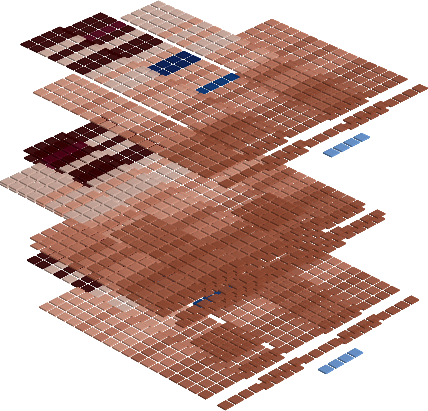
\includegraphics[width=1.5cm]{src/colorspace_colourflow/flows/colourflow_55-45.png}%           
  \end{adjustbox}                                                        
\caption*{

\begin{tikzpicture}                             
\definecolor{tempcolor}{HTML}{000000}           
\fill[tempcolor] (1 mm,0) rectangle ++(1mm,1mm);
\definecolor{tempcolor}{HTML}{b55d40}           
\fill[tempcolor] (2 mm,0) rectangle ++(1mm,1mm);
\definecolor{tempcolor}{HTML}{c66e51}           
\fill[tempcolor] (3 mm,0) rectangle ++(1mm,1mm);
\definecolor{tempcolor}{HTML}{e89073}           
\fill[tempcolor] (4 mm,0) rectangle ++(1mm,1mm);
\definecolor{tempcolor}{HTML}{ffb298}           
\fill[tempcolor] (5 mm,0) rectangle ++(1mm,1mm);
\definecolor{tempcolor}{HTML}{ffd4c4}           
\fill[tempcolor] (6 mm,0) rectangle ++(1mm,1mm);
\definecolor{tempcolor}{HTML}{410103}           
\fill[tempcolor] (7 mm,0) rectangle ++(1mm,1mm);
\definecolor{tempcolor}{HTML}{61001b}           
\fill[tempcolor] (8 mm,0) rectangle ++(1mm,1mm);
\end{tikzpicture}                               
}
\end{figure}                                                               
\end{minipage}
\hspace{0.1cm}
\begin{minipage}[b]{0.15\linewidth}
\begin{figure}[H]                                                          
  \centering                                                             
  \begin{adjustbox}{width=1.5cm,center}                                   
  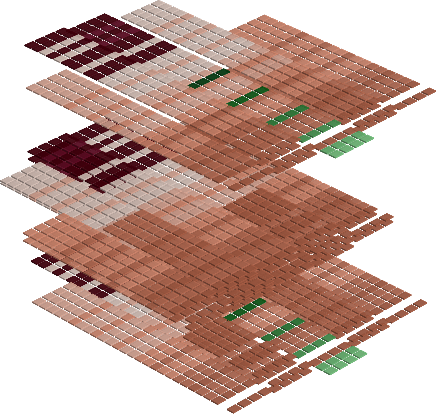
\includegraphics[width=1.5cm]{src/colorspace_colourflow/flows/colourflow_56-45.png}%           
  \end{adjustbox}                                                        
\caption*{

\begin{tikzpicture}                             
\definecolor{tempcolor}{HTML}{000000}           
\fill[tempcolor] (1 mm,0) rectangle ++(1mm,1mm);
\definecolor{tempcolor}{HTML}{c66e51}           
\fill[tempcolor] (2 mm,0) rectangle ++(1mm,1mm);
\definecolor{tempcolor}{HTML}{d77f62}           
\fill[tempcolor] (3 mm,0) rectangle ++(1mm,1mm);
\definecolor{tempcolor}{HTML}{f9a183}           
\fill[tempcolor] (4 mm,0) rectangle ++(1mm,1mm);
\definecolor{tempcolor}{HTML}{ffc3ae}           
\fill[tempcolor] (5 mm,0) rectangle ++(1mm,1mm);
\definecolor{tempcolor}{HTML}{ffe5da}           
\fill[tempcolor] (6 mm,0) rectangle ++(1mm,1mm);
\definecolor{tempcolor}{HTML}{50000f}           
\fill[tempcolor] (7 mm,0) rectangle ++(1mm,1mm);
\definecolor{tempcolor}{HTML}{720f2b}           
\fill[tempcolor] (8 mm,0) rectangle ++(1mm,1mm);
\end{tikzpicture}                               
}
\end{figure}                                                               
\end{minipage}
\hspace{0.1cm}
\begin{minipage}[b]{0.15\linewidth}
\begin{figure}[H]                                                          
  \centering                                                             
  \begin{adjustbox}{width=1.5cm,center}                                   
  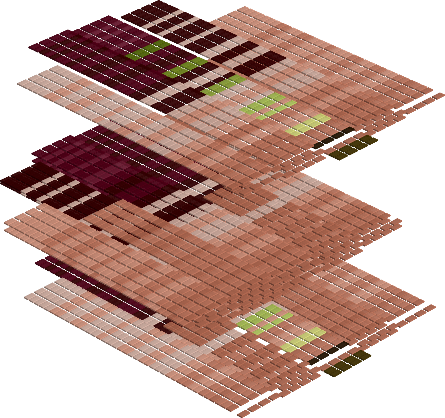
\includegraphics[width=1.5cm]{src/colorspace_colourflow/flows/colourflow_57-45.png}%           
  \end{adjustbox}                                                        
\caption*{

\begin{tikzpicture}                             
\definecolor{tempcolor}{HTML}{000000}           
\fill[tempcolor] (1 mm,0) rectangle ++(1mm,1mm);
\definecolor{tempcolor}{HTML}{d77f62}           
\fill[tempcolor] (2 mm,0) rectangle ++(1mm,1mm);
\definecolor{tempcolor}{HTML}{e89073}           
\fill[tempcolor] (3 mm,0) rectangle ++(1mm,1mm);
\definecolor{tempcolor}{HTML}{ffb298}           
\fill[tempcolor] (4 mm,0) rectangle ++(1mm,1mm);
\definecolor{tempcolor}{HTML}{ffd4c4}           
\fill[tempcolor] (5 mm,0) rectangle ++(1mm,1mm);
\definecolor{tempcolor}{HTML}{410103}           
\fill[tempcolor] (6 mm,0) rectangle ++(1mm,1mm);
\definecolor{tempcolor}{HTML}{61001b}           
\fill[tempcolor] (7 mm,0) rectangle ++(1mm,1mm);
\definecolor{tempcolor}{HTML}{83203c}           
\fill[tempcolor] (8 mm,0) rectangle ++(1mm,1mm);
\end{tikzpicture}                               
}
\end{figure}                                                               
\end{minipage}
\hspace{0.1cm}
\begin{minipage}[b]{0.15\linewidth}
\begin{figure}[H]                                                          
  \centering                                                             
  \begin{adjustbox}{width=1.5cm,center}                                   
  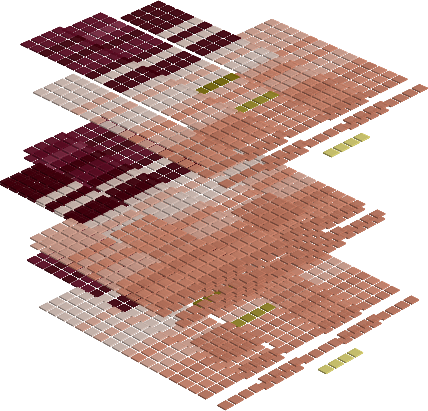
\includegraphics[width=1.5cm]{src/colorspace_colourflow/flows/colourflow_58-45.png}%           
  \end{adjustbox}                                                        
\caption*{

\begin{tikzpicture}                             
\definecolor{tempcolor}{HTML}{000000}           
\fill[tempcolor] (1 mm,0) rectangle ++(1mm,1mm);
\definecolor{tempcolor}{HTML}{e89073}           
\fill[tempcolor] (2 mm,0) rectangle ++(1mm,1mm);
\definecolor{tempcolor}{HTML}{f9a183}           
\fill[tempcolor] (3 mm,0) rectangle ++(1mm,1mm);
\definecolor{tempcolor}{HTML}{ffc3ae}           
\fill[tempcolor] (4 mm,0) rectangle ++(1mm,1mm);
\definecolor{tempcolor}{HTML}{ffe5da}           
\fill[tempcolor] (5 mm,0) rectangle ++(1mm,1mm);
\definecolor{tempcolor}{HTML}{50000f}           
\fill[tempcolor] (6 mm,0) rectangle ++(1mm,1mm);
\definecolor{tempcolor}{HTML}{720f2b}           
\fill[tempcolor] (7 mm,0) rectangle ++(1mm,1mm);
\definecolor{tempcolor}{HTML}{94314d}           
\fill[tempcolor] (8 mm,0) rectangle ++(1mm,1mm);
\end{tikzpicture}                               
}
\end{figure}                                                               
\end{minipage}
\hspace{0.1cm}
\begin{minipage}[b]{0.15\linewidth}
\begin{figure}[H]                                                          
  \centering                                                             
  \begin{adjustbox}{width=1.5cm,center}                                   
  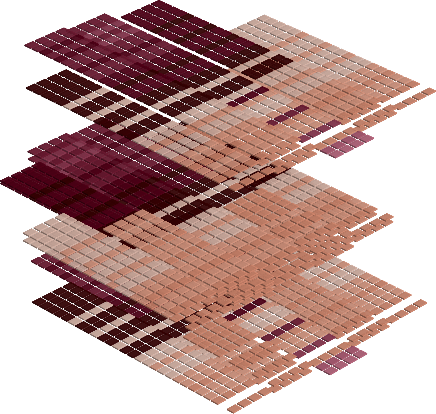
\includegraphics[width=1.5cm]{src/colorspace_colourflow/flows/colourflow_59-45.png}%           
  \end{adjustbox}                                                        
\caption*{

\begin{tikzpicture}                             
\definecolor{tempcolor}{HTML}{000000}           
\fill[tempcolor] (1 mm,0) rectangle ++(1mm,1mm);
\definecolor{tempcolor}{HTML}{f9a183}           
\fill[tempcolor] (2 mm,0) rectangle ++(1mm,1mm);
\definecolor{tempcolor}{HTML}{ffb298}           
\fill[tempcolor] (3 mm,0) rectangle ++(1mm,1mm);
\definecolor{tempcolor}{HTML}{ffd4c4}           
\fill[tempcolor] (4 mm,0) rectangle ++(1mm,1mm);
\definecolor{tempcolor}{HTML}{410103}           
\fill[tempcolor] (5 mm,0) rectangle ++(1mm,1mm);
\definecolor{tempcolor}{HTML}{61001b}           
\fill[tempcolor] (6 mm,0) rectangle ++(1mm,1mm);
\definecolor{tempcolor}{HTML}{83203c}           
\fill[tempcolor] (7 mm,0) rectangle ++(1mm,1mm);
\definecolor{tempcolor}{HTML}{a5425e}           
\fill[tempcolor] (8 mm,0) rectangle ++(1mm,1mm);
\end{tikzpicture}                               
}
\end{figure}                                                               
\end{minipage}
\hspace{0.1cm}
\begin{minipage}[b]{0.15\linewidth}
\begin{figure}[H]                                                          
  \centering                                                             
  \begin{adjustbox}{width=1.5cm,center}                                   
  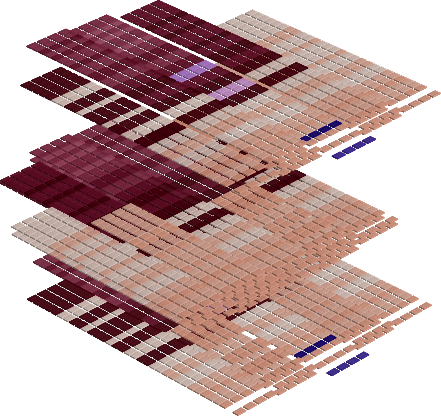
\includegraphics[width=1.5cm]{src/colorspace_colourflow/flows/colourflow_60-45.png}%           
  \end{adjustbox}                                                        
\caption*{

\begin{tikzpicture}                             
\definecolor{tempcolor}{HTML}{000000}           
\fill[tempcolor] (1 mm,0) rectangle ++(1mm,1mm);
\definecolor{tempcolor}{HTML}{ffb298}           
\fill[tempcolor] (2 mm,0) rectangle ++(1mm,1mm);
\definecolor{tempcolor}{HTML}{ffc3ae}           
\fill[tempcolor] (3 mm,0) rectangle ++(1mm,1mm);
\definecolor{tempcolor}{HTML}{ffe5da}           
\fill[tempcolor] (4 mm,0) rectangle ++(1mm,1mm);
\definecolor{tempcolor}{HTML}{50000f}           
\fill[tempcolor] (5 mm,0) rectangle ++(1mm,1mm);
\definecolor{tempcolor}{HTML}{720f2b}           
\fill[tempcolor] (6 mm,0) rectangle ++(1mm,1mm);
\definecolor{tempcolor}{HTML}{94314d}           
\fill[tempcolor] (7 mm,0) rectangle ++(1mm,1mm);
\definecolor{tempcolor}{HTML}{b6536f}           
\fill[tempcolor] (8 mm,0) rectangle ++(1mm,1mm);
\end{tikzpicture}                               
}
\end{figure}                                                               
\end{minipage}
\hspace{0.1cm}
\begin{minipage}[b]{0.15\linewidth}
\begin{figure}[H]                                                          
  \centering                                                             
  \begin{adjustbox}{width=1.5cm,center}                                   
  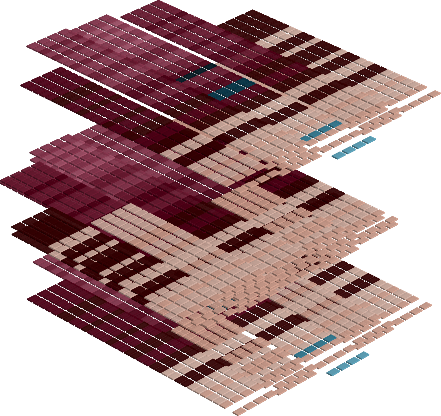
\includegraphics[width=1.5cm]{src/colorspace_colourflow/flows/colourflow_61-45.png}%           
  \end{adjustbox}                                                        
\caption*{

\begin{tikzpicture}                             
\definecolor{tempcolor}{HTML}{000000}           
\fill[tempcolor] (1 mm,0) rectangle ++(1mm,1mm);
\definecolor{tempcolor}{HTML}{ffc3ae}           
\fill[tempcolor] (2 mm,0) rectangle ++(1mm,1mm);
\definecolor{tempcolor}{HTML}{ffd4c4}           
\fill[tempcolor] (3 mm,0) rectangle ++(1mm,1mm);
\definecolor{tempcolor}{HTML}{410103}           
\fill[tempcolor] (4 mm,0) rectangle ++(1mm,1mm);
\definecolor{tempcolor}{HTML}{61001b}           
\fill[tempcolor] (5 mm,0) rectangle ++(1mm,1mm);
\definecolor{tempcolor}{HTML}{83203c}           
\fill[tempcolor] (6 mm,0) rectangle ++(1mm,1mm);
\definecolor{tempcolor}{HTML}{a5425e}           
\fill[tempcolor] (7 mm,0) rectangle ++(1mm,1mm);
\definecolor{tempcolor}{HTML}{c76480}           
\fill[tempcolor] (8 mm,0) rectangle ++(1mm,1mm);
\end{tikzpicture}                               
}
\end{figure}                                                               
\end{minipage}
\hspace{0.1cm}
\begin{minipage}[b]{0.15\linewidth}
\begin{figure}[H]                                                          
  \centering                                                             
  \begin{adjustbox}{width=1.5cm,center}                                   
  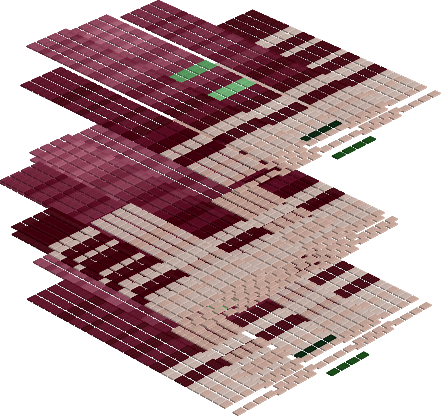
\includegraphics[width=1.5cm]{src/colorspace_colourflow/flows/colourflow_62-45.png}%           
  \end{adjustbox}                                                        
\caption*{

\begin{tikzpicture}                             
\definecolor{tempcolor}{HTML}{000000}           
\fill[tempcolor] (1 mm,0) rectangle ++(1mm,1mm);
\definecolor{tempcolor}{HTML}{ffd4c4}           
\fill[tempcolor] (2 mm,0) rectangle ++(1mm,1mm);
\definecolor{tempcolor}{HTML}{ffe5da}           
\fill[tempcolor] (3 mm,0) rectangle ++(1mm,1mm);
\definecolor{tempcolor}{HTML}{50000f}           
\fill[tempcolor] (4 mm,0) rectangle ++(1mm,1mm);
\definecolor{tempcolor}{HTML}{720f2b}           
\fill[tempcolor] (5 mm,0) rectangle ++(1mm,1mm);
\definecolor{tempcolor}{HTML}{94314d}           
\fill[tempcolor] (6 mm,0) rectangle ++(1mm,1mm);
\definecolor{tempcolor}{HTML}{b6536f}           
\fill[tempcolor] (7 mm,0) rectangle ++(1mm,1mm);
\definecolor{tempcolor}{HTML}{d87591}           
\fill[tempcolor] (8 mm,0) rectangle ++(1mm,1mm);
\end{tikzpicture}                               
}
\end{figure}                                                               
\end{minipage}
\hspace{0.1cm}
\begin{minipage}[b]{0.15\linewidth}
\begin{figure}[H]                                                          
  \centering                                                             
  \begin{adjustbox}{width=1.5cm,center}                                   
  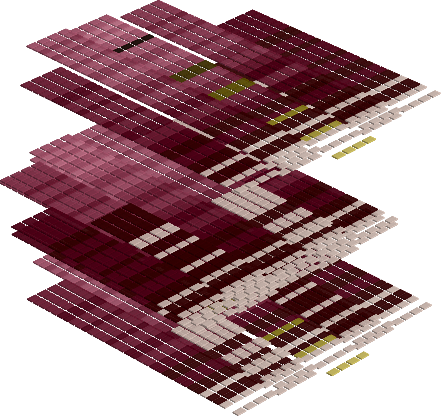
\includegraphics[width=1.5cm]{src/colorspace_colourflow/flows/colourflow_63-45.png}%           
  \end{adjustbox}                                                        
\caption*{

\begin{tikzpicture}                             
\definecolor{tempcolor}{HTML}{000000}           
\fill[tempcolor] (1 mm,0) rectangle ++(1mm,1mm);
\definecolor{tempcolor}{HTML}{ffe5da}           
\fill[tempcolor] (2 mm,0) rectangle ++(1mm,1mm);
\definecolor{tempcolor}{HTML}{410103}           
\fill[tempcolor] (3 mm,0) rectangle ++(1mm,1mm);
\definecolor{tempcolor}{HTML}{61001b}           
\fill[tempcolor] (4 mm,0) rectangle ++(1mm,1mm);
\definecolor{tempcolor}{HTML}{83203c}           
\fill[tempcolor] (5 mm,0) rectangle ++(1mm,1mm);
\definecolor{tempcolor}{HTML}{a5425e}           
\fill[tempcolor] (6 mm,0) rectangle ++(1mm,1mm);
\definecolor{tempcolor}{HTML}{c76480}           
\fill[tempcolor] (7 mm,0) rectangle ++(1mm,1mm);
\definecolor{tempcolor}{HTML}{e986a2}           
\fill[tempcolor] (8 mm,0) rectangle ++(1mm,1mm);
\end{tikzpicture}                               
}
\end{figure}                                                               
\end{minipage}
\hspace{0.1cm}
\begin{minipage}[b]{0.15\linewidth}
\begin{figure}[H]                                                          
  \centering                                                             
  \begin{adjustbox}{width=1.5cm,center}                                   
  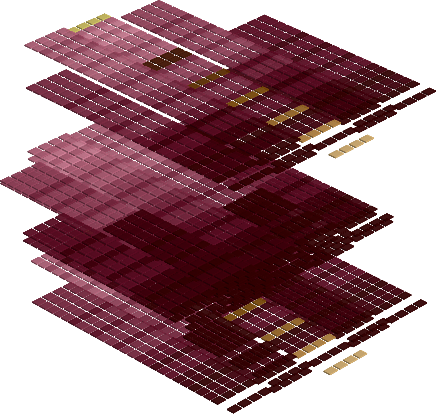
\includegraphics[width=1.5cm]{src/colorspace_colourflow/flows/colourflow_64-45.png}%           
  \end{adjustbox}                                                        
\caption*{

\begin{tikzpicture}                             
\definecolor{tempcolor}{HTML}{000000}           
\fill[tempcolor] (1 mm,0) rectangle ++(1mm,1mm);
\definecolor{tempcolor}{HTML}{410103}           
\fill[tempcolor] (2 mm,0) rectangle ++(1mm,1mm);
\definecolor{tempcolor}{HTML}{50000f}           
\fill[tempcolor] (3 mm,0) rectangle ++(1mm,1mm);
\definecolor{tempcolor}{HTML}{720f2b}           
\fill[tempcolor] (4 mm,0) rectangle ++(1mm,1mm);
\definecolor{tempcolor}{HTML}{94314d}           
\fill[tempcolor] (5 mm,0) rectangle ++(1mm,1mm);
\definecolor{tempcolor}{HTML}{b6536f}           
\fill[tempcolor] (6 mm,0) rectangle ++(1mm,1mm);
\definecolor{tempcolor}{HTML}{d87591}           
\fill[tempcolor] (7 mm,0) rectangle ++(1mm,1mm);
\definecolor{tempcolor}{HTML}{fa97b3}           
\fill[tempcolor] (8 mm,0) rectangle ++(1mm,1mm);
\end{tikzpicture}                               
}
\end{figure}                                                               
\end{minipage}
\hspace{0.1cm}
\begin{minipage}[b]{0.15\linewidth}
\begin{figure}[H]                                                          
  \centering                                                             
  \begin{adjustbox}{width=1.5cm,center}                                   
  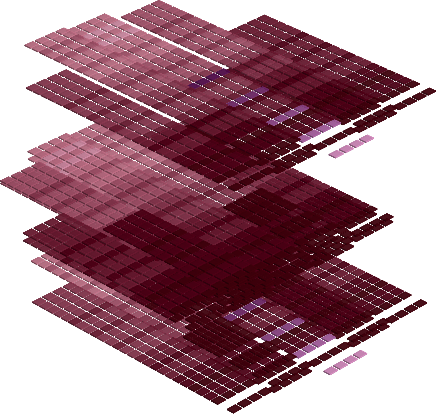
\includegraphics[width=1.5cm]{src/colorspace_colourflow/flows/colourflow_65-45.png}%           
  \end{adjustbox}                                                        
\caption*{

\begin{tikzpicture}                             
\definecolor{tempcolor}{HTML}{000000}           
\fill[tempcolor] (1 mm,0) rectangle ++(1mm,1mm);
\definecolor{tempcolor}{HTML}{50000f}           
\fill[tempcolor] (2 mm,0) rectangle ++(1mm,1mm);
\definecolor{tempcolor}{HTML}{61001b}           
\fill[tempcolor] (3 mm,0) rectangle ++(1mm,1mm);
\definecolor{tempcolor}{HTML}{83203c}           
\fill[tempcolor] (4 mm,0) rectangle ++(1mm,1mm);
\definecolor{tempcolor}{HTML}{a5425e}           
\fill[tempcolor] (5 mm,0) rectangle ++(1mm,1mm);
\definecolor{tempcolor}{HTML}{c76480}           
\fill[tempcolor] (6 mm,0) rectangle ++(1mm,1mm);
\definecolor{tempcolor}{HTML}{e986a2}           
\fill[tempcolor] (7 mm,0) rectangle ++(1mm,1mm);
\definecolor{tempcolor}{HTML}{ffa8c8}           
\fill[tempcolor] (8 mm,0) rectangle ++(1mm,1mm);
\end{tikzpicture}                               
}
\end{figure}                                                               
\end{minipage}
\hspace{0.1cm}
\begin{minipage}[b]{0.15\linewidth}
\begin{figure}[H]                                                          
  \centering                                                             
  \begin{adjustbox}{width=1.5cm,center}                                   
  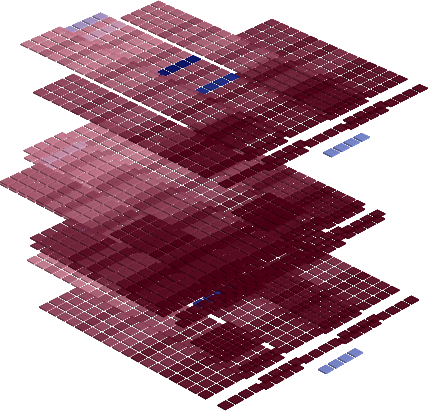
\includegraphics[width=1.5cm]{src/colorspace_colourflow/flows/colourflow_66-45.png}%           
  \end{adjustbox}                                                        
\caption*{

\begin{tikzpicture}                             
\definecolor{tempcolor}{HTML}{000000}           
\fill[tempcolor] (1 mm,0) rectangle ++(1mm,1mm);
\definecolor{tempcolor}{HTML}{61001b}           
\fill[tempcolor] (2 mm,0) rectangle ++(1mm,1mm);
\definecolor{tempcolor}{HTML}{720f2b}           
\fill[tempcolor] (3 mm,0) rectangle ++(1mm,1mm);
\definecolor{tempcolor}{HTML}{94314d}           
\fill[tempcolor] (4 mm,0) rectangle ++(1mm,1mm);
\definecolor{tempcolor}{HTML}{b6536f}           
\fill[tempcolor] (5 mm,0) rectangle ++(1mm,1mm);
\definecolor{tempcolor}{HTML}{d87591}           
\fill[tempcolor] (6 mm,0) rectangle ++(1mm,1mm);
\definecolor{tempcolor}{HTML}{fa97b3}           
\fill[tempcolor] (7 mm,0) rectangle ++(1mm,1mm);
\definecolor{tempcolor}{HTML}{ffb9de}           
\fill[tempcolor] (8 mm,0) rectangle ++(1mm,1mm);
\end{tikzpicture}                               
}
\end{figure}                                                               
\end{minipage}
\hspace{0.1cm}
\begin{minipage}[b]{0.15\linewidth}
\begin{figure}[H]                                                          
  \centering                                                             
  \begin{adjustbox}{width=1.5cm,center}                                   
  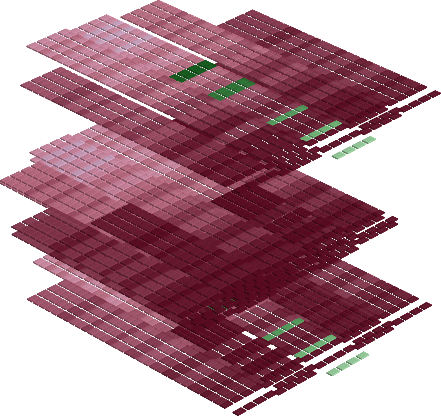
\includegraphics[width=1.5cm]{src/colorspace_colourflow/flows/colourflow_67-45.png}%           
  \end{adjustbox}                                                        
\caption*{

\begin{tikzpicture}                             
\definecolor{tempcolor}{HTML}{000000}           
\fill[tempcolor] (1 mm,0) rectangle ++(1mm,1mm);
\definecolor{tempcolor}{HTML}{720f2b}           
\fill[tempcolor] (2 mm,0) rectangle ++(1mm,1mm);
\definecolor{tempcolor}{HTML}{83203c}           
\fill[tempcolor] (3 mm,0) rectangle ++(1mm,1mm);
\definecolor{tempcolor}{HTML}{a5425e}           
\fill[tempcolor] (4 mm,0) rectangle ++(1mm,1mm);
\definecolor{tempcolor}{HTML}{c76480}           
\fill[tempcolor] (5 mm,0) rectangle ++(1mm,1mm);
\definecolor{tempcolor}{HTML}{e986a2}           
\fill[tempcolor] (6 mm,0) rectangle ++(1mm,1mm);
\definecolor{tempcolor}{HTML}{ffa8c8}           
\fill[tempcolor] (7 mm,0) rectangle ++(1mm,1mm);
\definecolor{tempcolor}{HTML}{ffcaef}           
\fill[tempcolor] (8 mm,0) rectangle ++(1mm,1mm);
\end{tikzpicture}                               
}
\end{figure}                                                               
\end{minipage}
\hspace{0.1cm}
\begin{minipage}[b]{0.15\linewidth}
\begin{figure}[H]                                                          
  \centering                                                             
  \begin{adjustbox}{width=1.5cm,center}                                   
  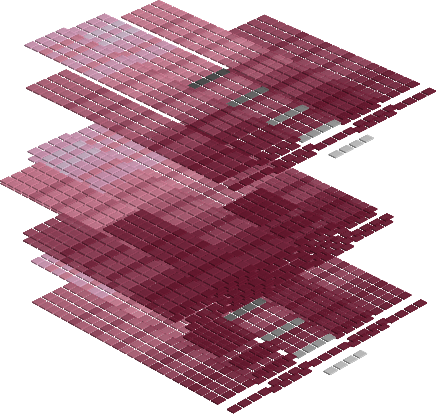
\includegraphics[width=1.5cm]{src/colorspace_colourflow/flows/colourflow_68-45.png}%           
  \end{adjustbox}                                                        
\caption*{

\begin{tikzpicture}                             
\definecolor{tempcolor}{HTML}{000000}           
\fill[tempcolor] (1 mm,0) rectangle ++(1mm,1mm);
\definecolor{tempcolor}{HTML}{83203c}           
\fill[tempcolor] (2 mm,0) rectangle ++(1mm,1mm);
\definecolor{tempcolor}{HTML}{94314d}           
\fill[tempcolor] (3 mm,0) rectangle ++(1mm,1mm);
\definecolor{tempcolor}{HTML}{b6536f}           
\fill[tempcolor] (4 mm,0) rectangle ++(1mm,1mm);
\definecolor{tempcolor}{HTML}{d87591}           
\fill[tempcolor] (5 mm,0) rectangle ++(1mm,1mm);
\definecolor{tempcolor}{HTML}{fa97b3}           
\fill[tempcolor] (6 mm,0) rectangle ++(1mm,1mm);
\definecolor{tempcolor}{HTML}{ffb9de}           
\fill[tempcolor] (7 mm,0) rectangle ++(1mm,1mm);
\definecolor{tempcolor}{HTML}{fbdcf6}           
\fill[tempcolor] (8 mm,0) rectangle ++(1mm,1mm);
\end{tikzpicture}                               
}
\end{figure}                                                               
\end{minipage}
\hspace{0.1cm}
\begin{minipage}[b]{0.15\linewidth}
\begin{figure}[H]                                                          
  \centering                                                             
  \begin{adjustbox}{width=1.5cm,center}                                   
  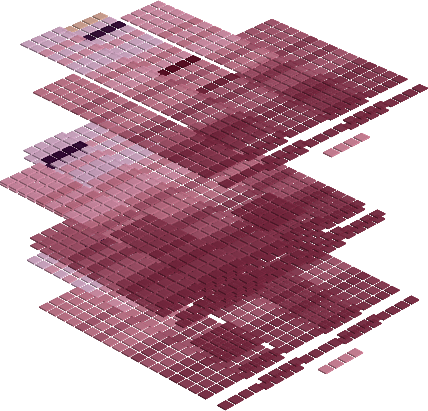
\includegraphics[width=1.5cm]{src/colorspace_colourflow/flows/colourflow_69-45.png}%           
  \end{adjustbox}                                                        
\caption*{

\begin{tikzpicture}                             
\definecolor{tempcolor}{HTML}{000000}           
\fill[tempcolor] (1 mm,0) rectangle ++(1mm,1mm);
\definecolor{tempcolor}{HTML}{94314d}           
\fill[tempcolor] (2 mm,0) rectangle ++(1mm,1mm);
\definecolor{tempcolor}{HTML}{a5425e}           
\fill[tempcolor] (3 mm,0) rectangle ++(1mm,1mm);
\definecolor{tempcolor}{HTML}{c76480}           
\fill[tempcolor] (4 mm,0) rectangle ++(1mm,1mm);
\definecolor{tempcolor}{HTML}{e986a2}           
\fill[tempcolor] (5 mm,0) rectangle ++(1mm,1mm);
\definecolor{tempcolor}{HTML}{ffa8c8}           
\fill[tempcolor] (6 mm,0) rectangle ++(1mm,1mm);
\definecolor{tempcolor}{HTML}{ffcaef}           
\fill[tempcolor] (7 mm,0) rectangle ++(1mm,1mm);
\definecolor{tempcolor}{HTML}{330035}           
\fill[tempcolor] (8 mm,0) rectangle ++(1mm,1mm);
\end{tikzpicture}                               
}
\end{figure}                                                               
\end{minipage}
\hspace{0.1cm}
\begin{minipage}[b]{0.15\linewidth}
\begin{figure}[H]                                                          
  \centering                                                             
  \begin{adjustbox}{width=1.5cm,center}                                   
  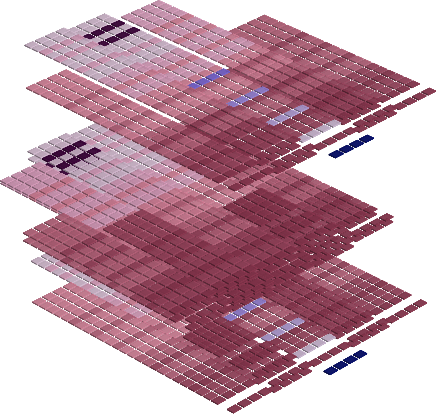
\includegraphics[width=1.5cm]{src/colorspace_colourflow/flows/colourflow_70-45.png}%           
  \end{adjustbox}                                                        
\caption*{

\begin{tikzpicture}                             
\definecolor{tempcolor}{HTML}{000000}           
\fill[tempcolor] (1 mm,0) rectangle ++(1mm,1mm);
\definecolor{tempcolor}{HTML}{a5425e}           
\fill[tempcolor] (2 mm,0) rectangle ++(1mm,1mm);
\definecolor{tempcolor}{HTML}{b6536f}           
\fill[tempcolor] (3 mm,0) rectangle ++(1mm,1mm);
\definecolor{tempcolor}{HTML}{d87591}           
\fill[tempcolor] (4 mm,0) rectangle ++(1mm,1mm);
\definecolor{tempcolor}{HTML}{fa97b3}           
\fill[tempcolor] (5 mm,0) rectangle ++(1mm,1mm);
\definecolor{tempcolor}{HTML}{ffb9de}           
\fill[tempcolor] (6 mm,0) rectangle ++(1mm,1mm);
\definecolor{tempcolor}{HTML}{fbdcf6}           
\fill[tempcolor] (7 mm,0) rectangle ++(1mm,1mm);
\definecolor{tempcolor}{HTML}{440041}           
\fill[tempcolor] (8 mm,0) rectangle ++(1mm,1mm);
\end{tikzpicture}                               
}
\end{figure}                                                               
\end{minipage}
\hspace{0.1cm}
\begin{minipage}[b]{0.15\linewidth}
\begin{figure}[H]                                                          
  \centering                                                             
  \begin{adjustbox}{width=1.5cm,center}                                   
  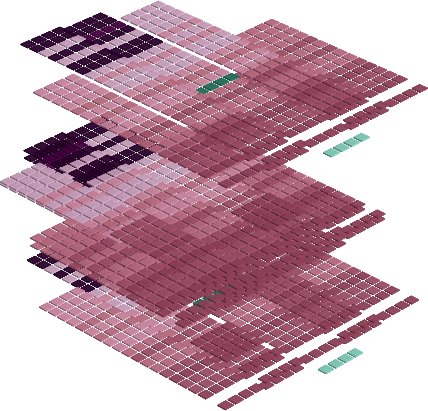
\includegraphics[width=1.5cm]{src/colorspace_colourflow/flows/colourflow_71-45.png}%           
  \end{adjustbox}                                                        
\caption*{

\begin{tikzpicture}                             
\definecolor{tempcolor}{HTML}{000000}           
\fill[tempcolor] (1 mm,0) rectangle ++(1mm,1mm);
\definecolor{tempcolor}{HTML}{b6536f}           
\fill[tempcolor] (2 mm,0) rectangle ++(1mm,1mm);
\definecolor{tempcolor}{HTML}{c76480}           
\fill[tempcolor] (3 mm,0) rectangle ++(1mm,1mm);
\definecolor{tempcolor}{HTML}{e986a2}           
\fill[tempcolor] (4 mm,0) rectangle ++(1mm,1mm);
\definecolor{tempcolor}{HTML}{ffa8c8}           
\fill[tempcolor] (5 mm,0) rectangle ++(1mm,1mm);
\definecolor{tempcolor}{HTML}{ffcaef}           
\fill[tempcolor] (6 mm,0) rectangle ++(1mm,1mm);
\definecolor{tempcolor}{HTML}{330035}           
\fill[tempcolor] (7 mm,0) rectangle ++(1mm,1mm);
\definecolor{tempcolor}{HTML}{55004c}           
\fill[tempcolor] (8 mm,0) rectangle ++(1mm,1mm);
\end{tikzpicture}                               
}
\end{figure}                                                               
\end{minipage}
\hspace{0.1cm}
\begin{minipage}[b]{0.15\linewidth}
\begin{figure}[H]                                                          
  \centering                                                             
  \begin{adjustbox}{width=1.5cm,center}                                   
  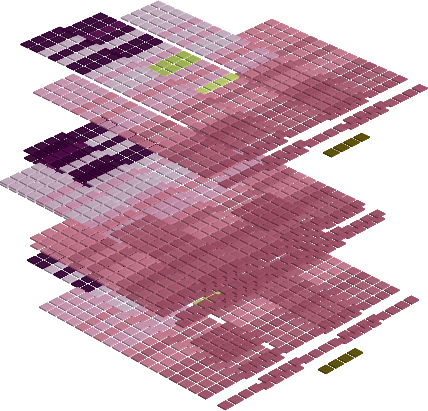
\includegraphics[width=1.5cm]{src/colorspace_colourflow/flows/colourflow_72-45.png}%           
  \end{adjustbox}                                                        
\caption*{

\begin{tikzpicture}                             
\definecolor{tempcolor}{HTML}{000000}           
\fill[tempcolor] (1 mm,0) rectangle ++(1mm,1mm);
\definecolor{tempcolor}{HTML}{c76480}           
\fill[tempcolor] (2 mm,0) rectangle ++(1mm,1mm);
\definecolor{tempcolor}{HTML}{d87591}           
\fill[tempcolor] (3 mm,0) rectangle ++(1mm,1mm);
\definecolor{tempcolor}{HTML}{fa97b3}           
\fill[tempcolor] (4 mm,0) rectangle ++(1mm,1mm);
\definecolor{tempcolor}{HTML}{ffb9de}           
\fill[tempcolor] (5 mm,0) rectangle ++(1mm,1mm);
\definecolor{tempcolor}{HTML}{fbdcf6}           
\fill[tempcolor] (6 mm,0) rectangle ++(1mm,1mm);
\definecolor{tempcolor}{HTML}{440041}           
\fill[tempcolor] (7 mm,0) rectangle ++(1mm,1mm);
\definecolor{tempcolor}{HTML}{660c5c}           
\fill[tempcolor] (8 mm,0) rectangle ++(1mm,1mm);
\end{tikzpicture}                               
}
\end{figure}                                                               
\end{minipage}
\hspace{0.1cm}
\begin{minipage}[b]{0.15\linewidth}
\begin{figure}[H]                                                          
  \centering                                                             
  \begin{adjustbox}{width=1.5cm,center}                                   
  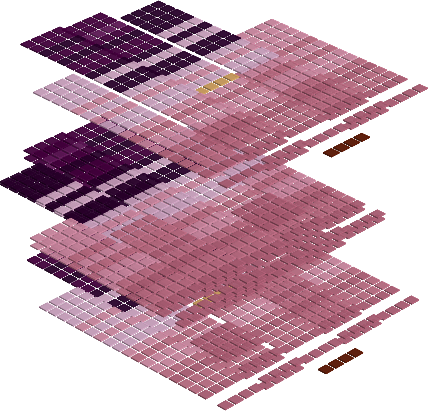
\includegraphics[width=1.5cm]{src/colorspace_colourflow/flows/colourflow_73-45.png}%           
  \end{adjustbox}                                                        
\caption*{

\begin{tikzpicture}                             
\definecolor{tempcolor}{HTML}{000000}           
\fill[tempcolor] (1 mm,0) rectangle ++(1mm,1mm);
\definecolor{tempcolor}{HTML}{d87591}           
\fill[tempcolor] (2 mm,0) rectangle ++(1mm,1mm);
\definecolor{tempcolor}{HTML}{e986a2}           
\fill[tempcolor] (3 mm,0) rectangle ++(1mm,1mm);
\definecolor{tempcolor}{HTML}{ffa8c8}           
\fill[tempcolor] (4 mm,0) rectangle ++(1mm,1mm);
\definecolor{tempcolor}{HTML}{ffcaef}           
\fill[tempcolor] (5 mm,0) rectangle ++(1mm,1mm);
\definecolor{tempcolor}{HTML}{330035}           
\fill[tempcolor] (6 mm,0) rectangle ++(1mm,1mm);
\definecolor{tempcolor}{HTML}{55004c}           
\fill[tempcolor] (7 mm,0) rectangle ++(1mm,1mm);
\definecolor{tempcolor}{HTML}{771d6d}           
\fill[tempcolor] (8 mm,0) rectangle ++(1mm,1mm);
\end{tikzpicture}                               
}
\end{figure}                                                               
\end{minipage}
\hspace{0.1cm}
\begin{minipage}[b]{0.15\linewidth}
\begin{figure}[H]                                                          
  \centering                                                             
  \begin{adjustbox}{width=1.5cm,center}                                   
  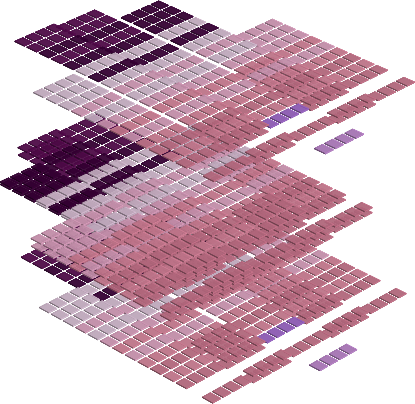
\includegraphics[width=1.5cm]{src/colorspace_colourflow/flows/colourflow_74-45.png}%           
  \end{adjustbox}                                                        
\caption*{

\begin{tikzpicture}                             
\definecolor{tempcolor}{HTML}{000000}           
\fill[tempcolor] (1 mm,0) rectangle ++(1mm,1mm);
\definecolor{tempcolor}{HTML}{e986a2}           
\fill[tempcolor] (2 mm,0) rectangle ++(1mm,1mm);
\definecolor{tempcolor}{HTML}{fa97b3}           
\fill[tempcolor] (3 mm,0) rectangle ++(1mm,1mm);
\definecolor{tempcolor}{HTML}{ffb9de}           
\fill[tempcolor] (4 mm,0) rectangle ++(1mm,1mm);
\definecolor{tempcolor}{HTML}{fbdcf6}           
\fill[tempcolor] (5 mm,0) rectangle ++(1mm,1mm);
\definecolor{tempcolor}{HTML}{440041}           
\fill[tempcolor] (6 mm,0) rectangle ++(1mm,1mm);
\definecolor{tempcolor}{HTML}{660c5c}           
\fill[tempcolor] (7 mm,0) rectangle ++(1mm,1mm);
\definecolor{tempcolor}{HTML}{882e7e}           
\fill[tempcolor] (8 mm,0) rectangle ++(1mm,1mm);
\end{tikzpicture}                               
}
\end{figure}                                                               
\end{minipage}
\hspace{0.1cm}
\begin{minipage}[b]{0.15\linewidth}
\begin{figure}[H]                                                          
  \centering                                                             
  \begin{adjustbox}{width=1.5cm,center}                                   
  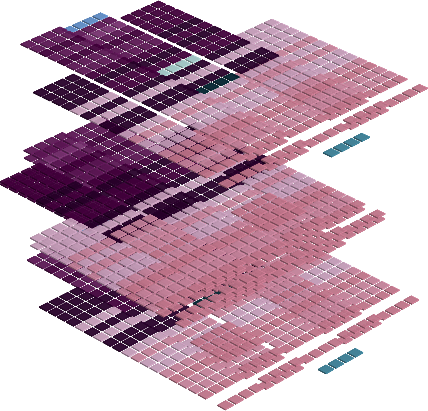
\includegraphics[width=1.5cm]{src/colorspace_colourflow/flows/colourflow_75-45.png}%           
  \end{adjustbox}                                                        
\caption*{

\begin{tikzpicture}                             
\definecolor{tempcolor}{HTML}{000000}           
\fill[tempcolor] (1 mm,0) rectangle ++(1mm,1mm);
\definecolor{tempcolor}{HTML}{fa97b3}           
\fill[tempcolor] (2 mm,0) rectangle ++(1mm,1mm);
\definecolor{tempcolor}{HTML}{ffa8c8}           
\fill[tempcolor] (3 mm,0) rectangle ++(1mm,1mm);
\definecolor{tempcolor}{HTML}{ffcaef}           
\fill[tempcolor] (4 mm,0) rectangle ++(1mm,1mm);
\definecolor{tempcolor}{HTML}{330035}           
\fill[tempcolor] (5 mm,0) rectangle ++(1mm,1mm);
\definecolor{tempcolor}{HTML}{55004c}           
\fill[tempcolor] (6 mm,0) rectangle ++(1mm,1mm);
\definecolor{tempcolor}{HTML}{771d6d}           
\fill[tempcolor] (7 mm,0) rectangle ++(1mm,1mm);
\definecolor{tempcolor}{HTML}{993f8f}           
\fill[tempcolor] (8 mm,0) rectangle ++(1mm,1mm);
\end{tikzpicture}                               
}
\end{figure}                                                               
\end{minipage}
\hspace{0.1cm}
\begin{minipage}[b]{0.15\linewidth}
\begin{figure}[H]                                                          
  \centering                                                             
  \begin{adjustbox}{width=1.5cm,center}                                   
  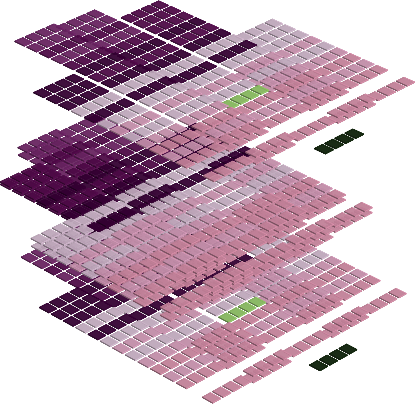
\includegraphics[width=1.5cm]{src/colorspace_colourflow/flows/colourflow_76-45.png}%           
  \end{adjustbox}                                                        
\caption*{

\begin{tikzpicture}                             
\definecolor{tempcolor}{HTML}{000000}           
\fill[tempcolor] (1 mm,0) rectangle ++(1mm,1mm);
\definecolor{tempcolor}{HTML}{ffa8c8}           
\fill[tempcolor] (2 mm,0) rectangle ++(1mm,1mm);
\definecolor{tempcolor}{HTML}{ffb9de}           
\fill[tempcolor] (3 mm,0) rectangle ++(1mm,1mm);
\definecolor{tempcolor}{HTML}{fbdcf6}           
\fill[tempcolor] (4 mm,0) rectangle ++(1mm,1mm);
\definecolor{tempcolor}{HTML}{440041}           
\fill[tempcolor] (5 mm,0) rectangle ++(1mm,1mm);
\definecolor{tempcolor}{HTML}{660c5c}           
\fill[tempcolor] (6 mm,0) rectangle ++(1mm,1mm);
\definecolor{tempcolor}{HTML}{882e7e}           
\fill[tempcolor] (7 mm,0) rectangle ++(1mm,1mm);
\definecolor{tempcolor}{HTML}{aa50a0}           
\fill[tempcolor] (8 mm,0) rectangle ++(1mm,1mm);
\end{tikzpicture}                               
}
\end{figure}                                                               
\end{minipage}
\hspace{0.1cm}
\begin{minipage}[b]{0.15\linewidth}
\begin{figure}[H]                                                          
  \centering                                                             
  \begin{adjustbox}{width=1.5cm,center}                                   
  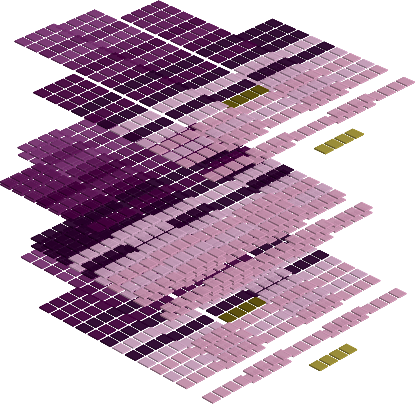
\includegraphics[width=1.5cm]{src/colorspace_colourflow/flows/colourflow_77-45.png}%           
  \end{adjustbox}                                                        
\caption*{

\begin{tikzpicture}                             
\definecolor{tempcolor}{HTML}{000000}           
\fill[tempcolor] (1 mm,0) rectangle ++(1mm,1mm);
\definecolor{tempcolor}{HTML}{ffb9de}           
\fill[tempcolor] (2 mm,0) rectangle ++(1mm,1mm);
\definecolor{tempcolor}{HTML}{ffcaef}           
\fill[tempcolor] (3 mm,0) rectangle ++(1mm,1mm);
\definecolor{tempcolor}{HTML}{330035}           
\fill[tempcolor] (4 mm,0) rectangle ++(1mm,1mm);
\definecolor{tempcolor}{HTML}{55004c}           
\fill[tempcolor] (5 mm,0) rectangle ++(1mm,1mm);
\definecolor{tempcolor}{HTML}{771d6d}           
\fill[tempcolor] (6 mm,0) rectangle ++(1mm,1mm);
\definecolor{tempcolor}{HTML}{993f8f}           
\fill[tempcolor] (7 mm,0) rectangle ++(1mm,1mm);
\definecolor{tempcolor}{HTML}{bb61b1}           
\fill[tempcolor] (8 mm,0) rectangle ++(1mm,1mm);
\end{tikzpicture}                               
}
\end{figure}                                                               
\end{minipage}
\hspace{0.1cm}
\begin{minipage}[b]{0.15\linewidth}
\begin{figure}[H]                                                          
  \centering                                                             
  \begin{adjustbox}{width=1.5cm,center}                                   
  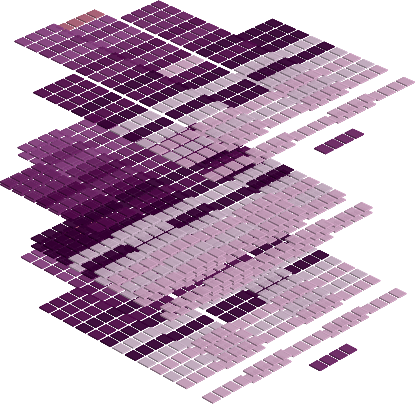
\includegraphics[width=1.5cm]{src/colorspace_colourflow/flows/colourflow_78-45.png}%           
  \end{adjustbox}                                                        
\caption*{

\begin{tikzpicture}                             
\definecolor{tempcolor}{HTML}{000000}           
\fill[tempcolor] (1 mm,0) rectangle ++(1mm,1mm);
\definecolor{tempcolor}{HTML}{ffcaef}           
\fill[tempcolor] (2 mm,0) rectangle ++(1mm,1mm);
\definecolor{tempcolor}{HTML}{fbdcf6}           
\fill[tempcolor] (3 mm,0) rectangle ++(1mm,1mm);
\definecolor{tempcolor}{HTML}{440041}           
\fill[tempcolor] (4 mm,0) rectangle ++(1mm,1mm);
\definecolor{tempcolor}{HTML}{660c5c}           
\fill[tempcolor] (5 mm,0) rectangle ++(1mm,1mm);
\definecolor{tempcolor}{HTML}{882e7e}           
\fill[tempcolor] (6 mm,0) rectangle ++(1mm,1mm);
\definecolor{tempcolor}{HTML}{aa50a0}           
\fill[tempcolor] (7 mm,0) rectangle ++(1mm,1mm);
\definecolor{tempcolor}{HTML}{cc72c2}           
\fill[tempcolor] (8 mm,0) rectangle ++(1mm,1mm);
\end{tikzpicture}                               
}
\end{figure}                                                               
\end{minipage}
\hspace{0.1cm}
\begin{minipage}[b]{0.15\linewidth}
\begin{figure}[H]                                                          
  \centering                                                             
  \begin{adjustbox}{width=1.5cm,center}                                   
  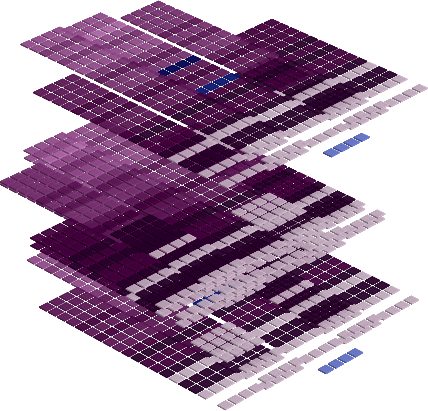
\includegraphics[width=1.5cm]{src/colorspace_colourflow/flows/colourflow_79-45.png}%           
  \end{adjustbox}                                                        
\caption*{

\begin{tikzpicture}                             
\definecolor{tempcolor}{HTML}{000000}           
\fill[tempcolor] (1 mm,0) rectangle ++(1mm,1mm);
\definecolor{tempcolor}{HTML}{fbdcf6}           
\fill[tempcolor] (2 mm,0) rectangle ++(1mm,1mm);
\definecolor{tempcolor}{HTML}{330035}           
\fill[tempcolor] (3 mm,0) rectangle ++(1mm,1mm);
\definecolor{tempcolor}{HTML}{55004c}           
\fill[tempcolor] (4 mm,0) rectangle ++(1mm,1mm);
\definecolor{tempcolor}{HTML}{771d6d}           
\fill[tempcolor] (5 mm,0) rectangle ++(1mm,1mm);
\definecolor{tempcolor}{HTML}{993f8f}           
\fill[tempcolor] (6 mm,0) rectangle ++(1mm,1mm);
\definecolor{tempcolor}{HTML}{bb61b1}           
\fill[tempcolor] (7 mm,0) rectangle ++(1mm,1mm);
\definecolor{tempcolor}{HTML}{dd83d3}           
\fill[tempcolor] (8 mm,0) rectangle ++(1mm,1mm);
\end{tikzpicture}                               
}
\end{figure}                                                               
\end{minipage}
\hspace{0.1cm}
\begin{minipage}[b]{0.15\linewidth}
\begin{figure}[H]                                                          
  \centering                                                             
  \begin{adjustbox}{width=1.5cm,center}                                   
  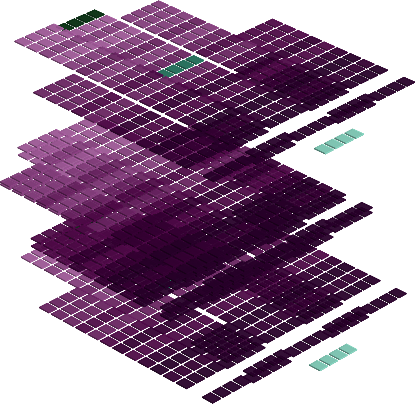
\includegraphics[width=1.5cm]{src/colorspace_colourflow/flows/colourflow_80-45.png}%           
  \end{adjustbox}                                                        
\caption*{

\begin{tikzpicture}                             
\definecolor{tempcolor}{HTML}{000000}           
\fill[tempcolor] (1 mm,0) rectangle ++(1mm,1mm);
\definecolor{tempcolor}{HTML}{330035}           
\fill[tempcolor] (2 mm,0) rectangle ++(1mm,1mm);
\definecolor{tempcolor}{HTML}{440041}           
\fill[tempcolor] (3 mm,0) rectangle ++(1mm,1mm);
\definecolor{tempcolor}{HTML}{660c5c}           
\fill[tempcolor] (4 mm,0) rectangle ++(1mm,1mm);
\definecolor{tempcolor}{HTML}{882e7e}           
\fill[tempcolor] (5 mm,0) rectangle ++(1mm,1mm);
\definecolor{tempcolor}{HTML}{aa50a0}           
\fill[tempcolor] (6 mm,0) rectangle ++(1mm,1mm);
\definecolor{tempcolor}{HTML}{cc72c2}           
\fill[tempcolor] (7 mm,0) rectangle ++(1mm,1mm);
\definecolor{tempcolor}{HTML}{ee94e4}           
\fill[tempcolor] (8 mm,0) rectangle ++(1mm,1mm);
\end{tikzpicture}                               
}
\end{figure}                                                               
\end{minipage}
\hspace{0.1cm}
\begin{minipage}[b]{0.15\linewidth}
\begin{figure}[H]                                                          
  \centering                                                             
  \begin{adjustbox}{width=1.5cm,center}                                   
  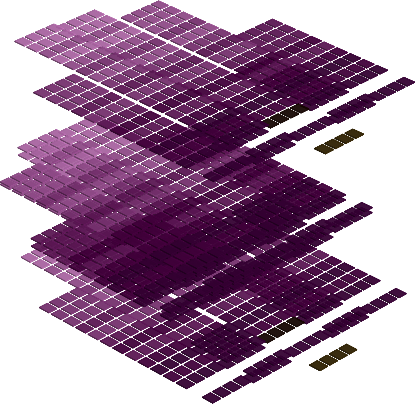
\includegraphics[width=1.5cm]{src/colorspace_colourflow/flows/colourflow_81-45.png}%           
  \end{adjustbox}                                                        
\caption*{

\begin{tikzpicture}                             
\definecolor{tempcolor}{HTML}{000000}           
\fill[tempcolor] (1 mm,0) rectangle ++(1mm,1mm);
\definecolor{tempcolor}{HTML}{440041}           
\fill[tempcolor] (2 mm,0) rectangle ++(1mm,1mm);
\definecolor{tempcolor}{HTML}{55004c}           
\fill[tempcolor] (3 mm,0) rectangle ++(1mm,1mm);
\definecolor{tempcolor}{HTML}{771d6d}           
\fill[tempcolor] (4 mm,0) rectangle ++(1mm,1mm);
\definecolor{tempcolor}{HTML}{993f8f}           
\fill[tempcolor] (5 mm,0) rectangle ++(1mm,1mm);
\definecolor{tempcolor}{HTML}{bb61b1}           
\fill[tempcolor] (6 mm,0) rectangle ++(1mm,1mm);
\definecolor{tempcolor}{HTML}{dd83d3}           
\fill[tempcolor] (7 mm,0) rectangle ++(1mm,1mm);
\definecolor{tempcolor}{HTML}{ffa5e4}           
\fill[tempcolor] (8 mm,0) rectangle ++(1mm,1mm);
\end{tikzpicture}                               
}
\end{figure}                                                               
\end{minipage}
\hspace{0.1cm}
\begin{minipage}[b]{0.15\linewidth}
\begin{figure}[H]                                                          
  \centering                                                             
  \begin{adjustbox}{width=1.5cm,center}                                   
  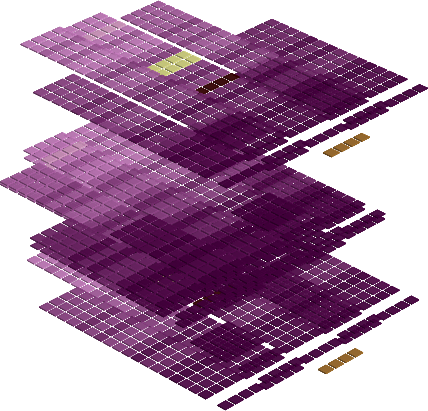
\includegraphics[width=1.5cm]{src/colorspace_colourflow/flows/colourflow_82-45.png}%           
  \end{adjustbox}                                                        
\caption*{

\begin{tikzpicture}                             
\definecolor{tempcolor}{HTML}{000000}           
\fill[tempcolor] (1 mm,0) rectangle ++(1mm,1mm);
\definecolor{tempcolor}{HTML}{55004c}           
\fill[tempcolor] (2 mm,0) rectangle ++(1mm,1mm);
\definecolor{tempcolor}{HTML}{660c5c}           
\fill[tempcolor] (3 mm,0) rectangle ++(1mm,1mm);
\definecolor{tempcolor}{HTML}{882e7e}           
\fill[tempcolor] (4 mm,0) rectangle ++(1mm,1mm);
\definecolor{tempcolor}{HTML}{aa50a0}           
\fill[tempcolor] (5 mm,0) rectangle ++(1mm,1mm);
\definecolor{tempcolor}{HTML}{cc72c2}           
\fill[tempcolor] (6 mm,0) rectangle ++(1mm,1mm);
\definecolor{tempcolor}{HTML}{ee94e4}           
\fill[tempcolor] (7 mm,0) rectangle ++(1mm,1mm);
\definecolor{tempcolor}{HTML}{ffb6e9}           
\fill[tempcolor] (8 mm,0) rectangle ++(1mm,1mm);
\end{tikzpicture}                               
}
\end{figure}                                                               
\end{minipage}
\hspace{0.1cm}
\begin{minipage}[b]{0.15\linewidth}
\begin{figure}[H]                                                          
  \centering                                                             
  \begin{adjustbox}{width=1.45cm,center}                                   
  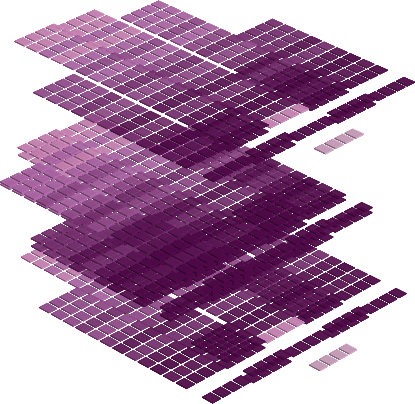
\includegraphics[width=1.45cm]{src/colorspace_colourflow/flows/colourflow_83-45.png}%           
  \end{adjustbox}                                                        
\caption*{

\begin{tikzpicture}                             
\definecolor{tempcolor}{HTML}{000000}           
\fill[tempcolor] (1 mm,0) rectangle ++(1mm,1mm);
\definecolor{tempcolor}{HTML}{660c5c}           
\fill[tempcolor] (2 mm,0) rectangle ++(1mm,1mm);
\definecolor{tempcolor}{HTML}{771d6d}           
\fill[tempcolor] (3 mm,0) rectangle ++(1mm,1mm);
\definecolor{tempcolor}{HTML}{993f8f}           
\fill[tempcolor] (4 mm,0) rectangle ++(1mm,1mm);
\definecolor{tempcolor}{HTML}{bb61b1}           
\fill[tempcolor] (5 mm,0) rectangle ++(1mm,1mm);
\definecolor{tempcolor}{HTML}{dd83d3}           
\fill[tempcolor] (6 mm,0) rectangle ++(1mm,1mm);
\definecolor{tempcolor}{HTML}{ffa5e4}           
\fill[tempcolor] (7 mm,0) rectangle ++(1mm,1mm);
\definecolor{tempcolor}{HTML}{ffc7ee}           
\fill[tempcolor] (8 mm,0) rectangle ++(1mm,1mm);
\end{tikzpicture}                               
}
\end{figure}                                                               
\end{minipage}
\hspace{0.1cm}
\begin{minipage}[b]{0.15\linewidth}
\begin{figure}[H]                                                          
  \centering                                                             
  \begin{adjustbox}{width=1.45cm,center}                                   
  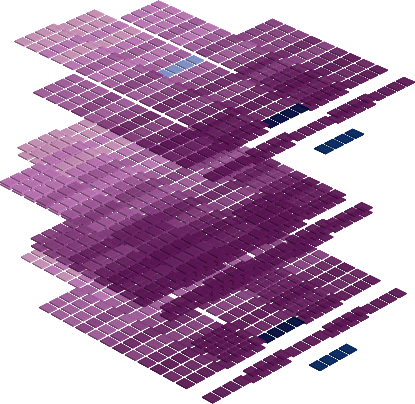
\includegraphics[width=1.45cm]{src/colorspace_colourflow/flows/colourflow_84-45.png}%           
  \end{adjustbox}                                                        
\caption*{

\begin{tikzpicture}                             
\definecolor{tempcolor}{HTML}{000000}           
\fill[tempcolor] (1 mm,0) rectangle ++(1mm,1mm);
\definecolor{tempcolor}{HTML}{771d6d}           
\fill[tempcolor] (2 mm,0) rectangle ++(1mm,1mm);
\definecolor{tempcolor}{HTML}{882e7e}           
\fill[tempcolor] (3 mm,0) rectangle ++(1mm,1mm);
\definecolor{tempcolor}{HTML}{aa50a0}           
\fill[tempcolor] (4 mm,0) rectangle ++(1mm,1mm);
\definecolor{tempcolor}{HTML}{cc72c2}           
\fill[tempcolor] (5 mm,0) rectangle ++(1mm,1mm);
\definecolor{tempcolor}{HTML}{ee94e4}           
\fill[tempcolor] (6 mm,0) rectangle ++(1mm,1mm);
\definecolor{tempcolor}{HTML}{ffb6e9}           
\fill[tempcolor] (7 mm,0) rectangle ++(1mm,1mm);
\definecolor{tempcolor}{HTML}{ffd8f3}           
\fill[tempcolor] (8 mm,0) rectangle ++(1mm,1mm);
\end{tikzpicture}                               
}
\end{figure}                                                               
\end{minipage}
\hspace{0.1cm}
\begin{minipage}[b]{0.15\linewidth}
\begin{figure}[H]                                                          
  \centering                                                             
  \begin{adjustbox}{width=1.45cm,center}                                   
  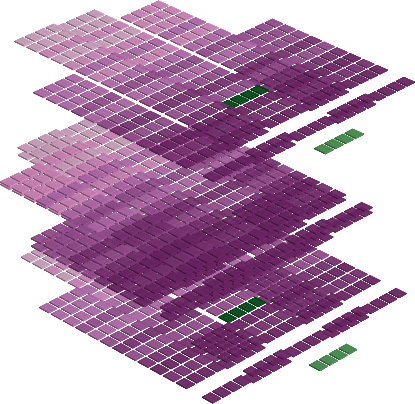
\includegraphics[width=1.45cm]{src/colorspace_colourflow/flows/colourflow_85-45.png}%           
  \end{adjustbox}                                                        
\caption*{

\begin{tikzpicture}                             
\definecolor{tempcolor}{HTML}{000000}           
\fill[tempcolor] (1 mm,0) rectangle ++(1mm,1mm);
\definecolor{tempcolor}{HTML}{882e7e}           
\fill[tempcolor] (2 mm,0) rectangle ++(1mm,1mm);
\definecolor{tempcolor}{HTML}{993f8f}           
\fill[tempcolor] (3 mm,0) rectangle ++(1mm,1mm);
\definecolor{tempcolor}{HTML}{bb61b1}           
\fill[tempcolor] (4 mm,0) rectangle ++(1mm,1mm);
\definecolor{tempcolor}{HTML}{dd83d3}           
\fill[tempcolor] (5 mm,0) rectangle ++(1mm,1mm);
\definecolor{tempcolor}{HTML}{ffa5e4}           
\fill[tempcolor] (6 mm,0) rectangle ++(1mm,1mm);
\definecolor{tempcolor}{HTML}{ffc7ee}           
\fill[tempcolor] (7 mm,0) rectangle ++(1mm,1mm);
\definecolor{tempcolor}{HTML}{1d005c}           
\fill[tempcolor] (8 mm,0) rectangle ++(1mm,1mm);
\end{tikzpicture}                               
}
\end{figure}                                                               
\end{minipage}
\hspace{0.1cm}
\begin{minipage}[b]{0.15\linewidth}
\begin{figure}[H]                                                          
  \centering                                                             
  \begin{adjustbox}{width=1.45cm,center}                                   
  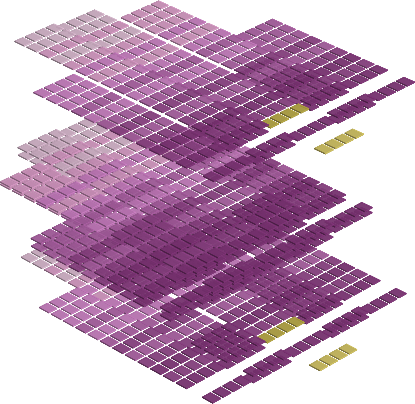
\includegraphics[width=1.45cm]{src/colorspace_colourflow/flows/colourflow_86-45.png}%           
  \end{adjustbox}                                                        
\caption*{

\begin{tikzpicture}                             
\definecolor{tempcolor}{HTML}{000000}           
\fill[tempcolor] (1 mm,0) rectangle ++(1mm,1mm);
\definecolor{tempcolor}{HTML}{993f8f}           
\fill[tempcolor] (2 mm,0) rectangle ++(1mm,1mm);
\definecolor{tempcolor}{HTML}{aa50a0}           
\fill[tempcolor] (3 mm,0) rectangle ++(1mm,1mm);
\definecolor{tempcolor}{HTML}{cc72c2}           
\fill[tempcolor] (4 mm,0) rectangle ++(1mm,1mm);
\definecolor{tempcolor}{HTML}{ee94e4}           
\fill[tempcolor] (5 mm,0) rectangle ++(1mm,1mm);
\definecolor{tempcolor}{HTML}{ffb6e9}           
\fill[tempcolor] (6 mm,0) rectangle ++(1mm,1mm);
\definecolor{tempcolor}{HTML}{ffd8f3}           
\fill[tempcolor] (7 mm,0) rectangle ++(1mm,1mm);
\definecolor{tempcolor}{HTML}{2e0068}           
\fill[tempcolor] (8 mm,0) rectangle ++(1mm,1mm);
\end{tikzpicture}                               
}
\end{figure}                                                               
\end{minipage}
\hspace{0.1cm}
\begin{minipage}[b]{0.15\linewidth}
\begin{figure}[H]                                                          
  \centering                                                             
  \begin{adjustbox}{width=1.45cm,center}                                   
  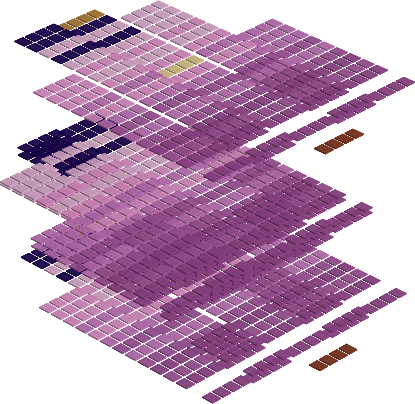
\includegraphics[width=1.45cm]{src/colorspace_colourflow/flows/colourflow_87-45.png}%           
  \end{adjustbox}                                                        
\caption*{

\begin{tikzpicture}                             
\definecolor{tempcolor}{HTML}{000000}           
\fill[tempcolor] (1 mm,0) rectangle ++(1mm,1mm);
\definecolor{tempcolor}{HTML}{aa50a0}           
\fill[tempcolor] (2 mm,0) rectangle ++(1mm,1mm);
\definecolor{tempcolor}{HTML}{bb61b1}           
\fill[tempcolor] (3 mm,0) rectangle ++(1mm,1mm);
\definecolor{tempcolor}{HTML}{dd83d3}           
\fill[tempcolor] (4 mm,0) rectangle ++(1mm,1mm);
\definecolor{tempcolor}{HTML}{ffa5e4}           
\fill[tempcolor] (5 mm,0) rectangle ++(1mm,1mm);
\definecolor{tempcolor}{HTML}{ffc7ee}           
\fill[tempcolor] (6 mm,0) rectangle ++(1mm,1mm);
\definecolor{tempcolor}{HTML}{1d005c}           
\fill[tempcolor] (7 mm,0) rectangle ++(1mm,1mm);
\definecolor{tempcolor}{HTML}{400074}           
\fill[tempcolor] (8 mm,0) rectangle ++(1mm,1mm);
\end{tikzpicture}                               
}
\end{figure}                                                               
\end{minipage}
\hspace{0.1cm}
\begin{minipage}[b]{0.15\linewidth}
\begin{figure}[H]                                                          
  \centering                                                             
  \begin{adjustbox}{width=1.45cm,center}                                   
  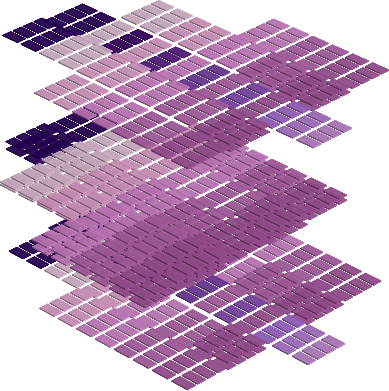
\includegraphics[width=1.45cm]{src/colorspace_colourflow/flows/colourflow_88-45.png}%           
  \end{adjustbox}                                                        
\caption*{

\begin{tikzpicture}                             
\definecolor{tempcolor}{HTML}{000000}           
\fill[tempcolor] (1 mm,0) rectangle ++(1mm,1mm);
\definecolor{tempcolor}{HTML}{bb61b1}           
\fill[tempcolor] (2 mm,0) rectangle ++(1mm,1mm);
\definecolor{tempcolor}{HTML}{cc72c2}           
\fill[tempcolor] (3 mm,0) rectangle ++(1mm,1mm);
\definecolor{tempcolor}{HTML}{ee94e4}           
\fill[tempcolor] (4 mm,0) rectangle ++(1mm,1mm);
\definecolor{tempcolor}{HTML}{ffb6e9}           
\fill[tempcolor] (5 mm,0) rectangle ++(1mm,1mm);
\definecolor{tempcolor}{HTML}{ffd8f3}           
\fill[tempcolor] (6 mm,0) rectangle ++(1mm,1mm);
\definecolor{tempcolor}{HTML}{2e0068}           
\fill[tempcolor] (7 mm,0) rectangle ++(1mm,1mm);
\definecolor{tempcolor}{HTML}{511084}           
\fill[tempcolor] (8 mm,0) rectangle ++(1mm,1mm);
\end{tikzpicture}                               
}
\end{figure}                                                               
\end{minipage}
\hspace{0.1cm}
\begin{minipage}[b]{0.15\linewidth}
\begin{figure}[H]                                                          
  \centering                                                             
  \begin{adjustbox}{width=1.45cm,center}                                   
  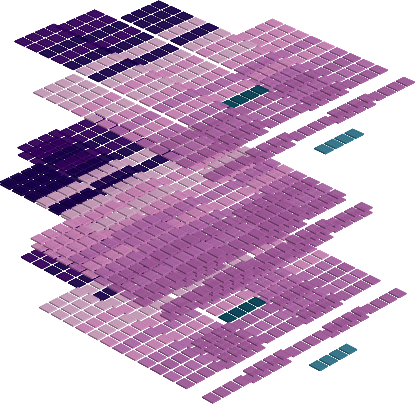
\includegraphics[width=1.45cm]{src/colorspace_colourflow/flows/colourflow_89-45.png}%           
  \end{adjustbox}                                                        
\caption*{

\begin{tikzpicture}                             
\definecolor{tempcolor}{HTML}{000000}           
\fill[tempcolor] (1 mm,0) rectangle ++(1mm,1mm);
\definecolor{tempcolor}{HTML}{cc72c2}           
\fill[tempcolor] (2 mm,0) rectangle ++(1mm,1mm);
\definecolor{tempcolor}{HTML}{dd83d3}           
\fill[tempcolor] (3 mm,0) rectangle ++(1mm,1mm);
\definecolor{tempcolor}{HTML}{ffa5e4}           
\fill[tempcolor] (4 mm,0) rectangle ++(1mm,1mm);
\definecolor{tempcolor}{HTML}{ffc7ee}           
\fill[tempcolor] (5 mm,0) rectangle ++(1mm,1mm);
\definecolor{tempcolor}{HTML}{1d005c}           
\fill[tempcolor] (6 mm,0) rectangle ++(1mm,1mm);
\definecolor{tempcolor}{HTML}{400074}           
\fill[tempcolor] (7 mm,0) rectangle ++(1mm,1mm);
\definecolor{tempcolor}{HTML}{622195}           
\fill[tempcolor] (8 mm,0) rectangle ++(1mm,1mm);
\end{tikzpicture}                               
}
\end{figure}                                                               
\end{minipage}
\hspace{0.1cm}
\begin{minipage}[b]{0.15\linewidth}
\begin{figure}[H]                                                          
  \centering                                                             
  \begin{adjustbox}{width=1.45cm,center}                                   
  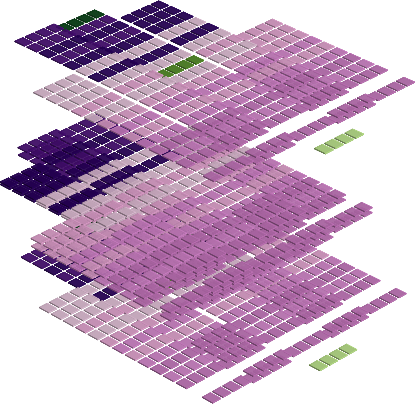
\includegraphics[width=1.45cm]{src/colorspace_colourflow/flows/colourflow_90-45.png}%           
  \end{adjustbox}                                                        
\caption*{

\begin{tikzpicture}                             
\definecolor{tempcolor}{HTML}{000000}           
\fill[tempcolor] (1 mm,0) rectangle ++(1mm,1mm);
\definecolor{tempcolor}{HTML}{dd83d3}           
\fill[tempcolor] (2 mm,0) rectangle ++(1mm,1mm);
\definecolor{tempcolor}{HTML}{ee94e4}           
\fill[tempcolor] (3 mm,0) rectangle ++(1mm,1mm);
\definecolor{tempcolor}{HTML}{ffb6e9}           
\fill[tempcolor] (4 mm,0) rectangle ++(1mm,1mm);
\definecolor{tempcolor}{HTML}{ffd8f3}           
\fill[tempcolor] (5 mm,0) rectangle ++(1mm,1mm);
\definecolor{tempcolor}{HTML}{2e0068}           
\fill[tempcolor] (6 mm,0) rectangle ++(1mm,1mm);
\definecolor{tempcolor}{HTML}{511084}           
\fill[tempcolor] (7 mm,0) rectangle ++(1mm,1mm);
\definecolor{tempcolor}{HTML}{7332a6}           
\fill[tempcolor] (8 mm,0) rectangle ++(1mm,1mm);
\end{tikzpicture}                               
}
\end{figure}                                                               
\end{minipage}
\hspace{0.1cm}
\begin{minipage}[b]{0.15\linewidth}
\begin{figure}[H]                                                          
  \centering                                                             
  \begin{adjustbox}{width=1.45cm,center}                                   
  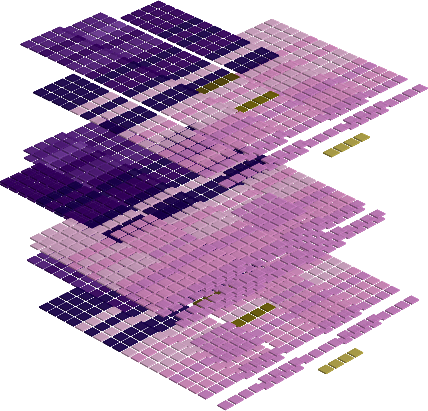
\includegraphics[width=1.45cm]{src/colorspace_colourflow/flows/colourflow_91-45.png}%           
  \end{adjustbox}                                                        
\caption*{

\begin{tikzpicture}                             
\definecolor{tempcolor}{HTML}{000000}           
\fill[tempcolor] (1 mm,0) rectangle ++(1mm,1mm);
\definecolor{tempcolor}{HTML}{ee94e4}           
\fill[tempcolor] (2 mm,0) rectangle ++(1mm,1mm);
\definecolor{tempcolor}{HTML}{ffa5e4}           
\fill[tempcolor] (3 mm,0) rectangle ++(1mm,1mm);
\definecolor{tempcolor}{HTML}{ffc7ee}           
\fill[tempcolor] (4 mm,0) rectangle ++(1mm,1mm);
\definecolor{tempcolor}{HTML}{1d005c}           
\fill[tempcolor] (5 mm,0) rectangle ++(1mm,1mm);
\definecolor{tempcolor}{HTML}{400074}           
\fill[tempcolor] (6 mm,0) rectangle ++(1mm,1mm);
\definecolor{tempcolor}{HTML}{622195}           
\fill[tempcolor] (7 mm,0) rectangle ++(1mm,1mm);
\definecolor{tempcolor}{HTML}{8443b7}           
\fill[tempcolor] (8 mm,0) rectangle ++(1mm,1mm);
\end{tikzpicture}                               
}
\end{figure}                                                               
\end{minipage}
\hspace{0.1cm}
\begin{minipage}[b]{0.15\linewidth}
\begin{figure}[H]                                                          
  \centering                                                             
  \begin{adjustbox}{width=1.45cm,center}                                   
  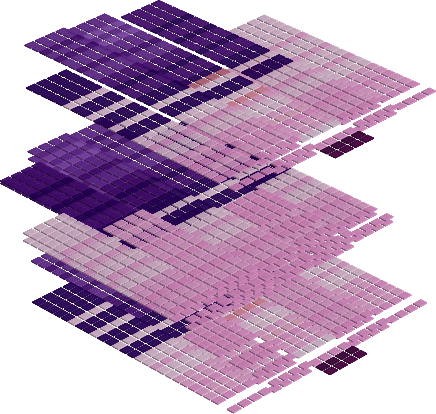
\includegraphics[width=1.45cm]{src/colorspace_colourflow/flows/colourflow_92-45.png}%           
  \end{adjustbox}                                                        
\caption*{

\begin{tikzpicture}                             
\definecolor{tempcolor}{HTML}{000000}           
\fill[tempcolor] (1 mm,0) rectangle ++(1mm,1mm);
\definecolor{tempcolor}{HTML}{ffa5e4}           
\fill[tempcolor] (2 mm,0) rectangle ++(1mm,1mm);
\definecolor{tempcolor}{HTML}{ffb6e9}           
\fill[tempcolor] (3 mm,0) rectangle ++(1mm,1mm);
\definecolor{tempcolor}{HTML}{ffd8f3}           
\fill[tempcolor] (4 mm,0) rectangle ++(1mm,1mm);
\definecolor{tempcolor}{HTML}{2e0068}           
\fill[tempcolor] (5 mm,0) rectangle ++(1mm,1mm);
\definecolor{tempcolor}{HTML}{511084}           
\fill[tempcolor] (6 mm,0) rectangle ++(1mm,1mm);
\definecolor{tempcolor}{HTML}{7332a6}           
\fill[tempcolor] (7 mm,0) rectangle ++(1mm,1mm);
\definecolor{tempcolor}{HTML}{9554c8}           
\fill[tempcolor] (8 mm,0) rectangle ++(1mm,1mm);
\end{tikzpicture}                               
}
\end{figure}                                                               
\end{minipage}
\hspace{0.1cm}
\begin{minipage}[b]{0.15\linewidth}
\begin{figure}[H]                                                          
  \centering                                                             
  \begin{adjustbox}{width=1.45cm,center}                                   
  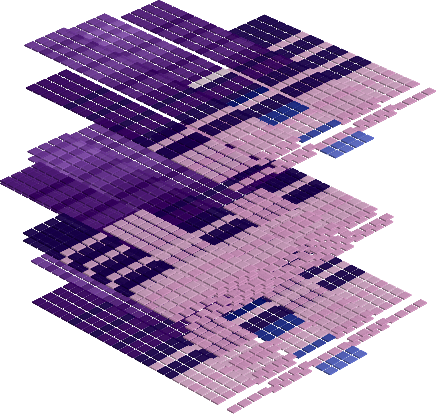
\includegraphics[width=1.45cm]{src/colorspace_colourflow/flows/colourflow_93-45.png}%           
  \end{adjustbox}                                                        
\caption*{

\begin{tikzpicture}                             
\definecolor{tempcolor}{HTML}{000000}           
\fill[tempcolor] (1 mm,0) rectangle ++(1mm,1mm);
\definecolor{tempcolor}{HTML}{ffb6e9}           
\fill[tempcolor] (2 mm,0) rectangle ++(1mm,1mm);
\definecolor{tempcolor}{HTML}{ffc7ee}           
\fill[tempcolor] (3 mm,0) rectangle ++(1mm,1mm);
\definecolor{tempcolor}{HTML}{1d005c}           
\fill[tempcolor] (4 mm,0) rectangle ++(1mm,1mm);
\definecolor{tempcolor}{HTML}{400074}           
\fill[tempcolor] (5 mm,0) rectangle ++(1mm,1mm);
\definecolor{tempcolor}{HTML}{622195}           
\fill[tempcolor] (6 mm,0) rectangle ++(1mm,1mm);
\definecolor{tempcolor}{HTML}{8443b7}           
\fill[tempcolor] (7 mm,0) rectangle ++(1mm,1mm);
\definecolor{tempcolor}{HTML}{a665d9}           
\fill[tempcolor] (8 mm,0) rectangle ++(1mm,1mm);
\end{tikzpicture}                               
}
\end{figure}                                                               
\end{minipage}
\hspace{0.1cm}
\begin{minipage}[b]{0.15\linewidth}
\begin{figure}[H]                                                          
  \centering                                                             
  \begin{adjustbox}{width=1.45cm,center}                                   
  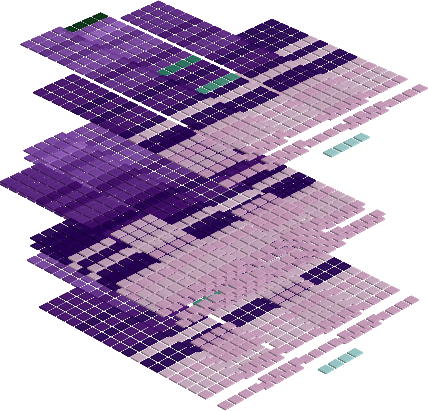
\includegraphics[width=1.45cm]{src/colorspace_colourflow/flows/colourflow_94-45.png}%           
  \end{adjustbox}                                                        
\caption*{

\begin{tikzpicture}                             
\definecolor{tempcolor}{HTML}{000000}           
\fill[tempcolor] (1 mm,0) rectangle ++(1mm,1mm);
\definecolor{tempcolor}{HTML}{ffc7ee}           
\fill[tempcolor] (2 mm,0) rectangle ++(1mm,1mm);
\definecolor{tempcolor}{HTML}{ffd8f3}           
\fill[tempcolor] (3 mm,0) rectangle ++(1mm,1mm);
\definecolor{tempcolor}{HTML}{2e0068}           
\fill[tempcolor] (4 mm,0) rectangle ++(1mm,1mm);
\definecolor{tempcolor}{HTML}{511084}           
\fill[tempcolor] (5 mm,0) rectangle ++(1mm,1mm);
\definecolor{tempcolor}{HTML}{7332a6}           
\fill[tempcolor] (6 mm,0) rectangle ++(1mm,1mm);
\definecolor{tempcolor}{HTML}{9554c8}           
\fill[tempcolor] (7 mm,0) rectangle ++(1mm,1mm);
\definecolor{tempcolor}{HTML}{b776ea}           
\fill[tempcolor] (8 mm,0) rectangle ++(1mm,1mm);
\end{tikzpicture}                               
}
\end{figure}                                                               
\end{minipage}
\hspace{0.1cm}
\begin{minipage}[b]{0.15\linewidth}
\begin{figure}[H]                                                          
  \centering                                                             
  \begin{adjustbox}{width=1.45cm,center}                                   
  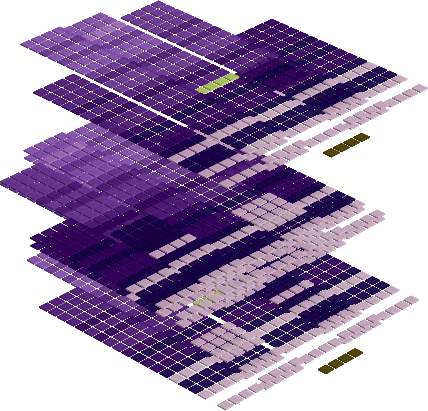
\includegraphics[width=1.45cm]{src/colorspace_colourflow/flows/colourflow_95-45.png}%           
  \end{adjustbox}                                                        
\caption*{

\begin{tikzpicture}                             
\definecolor{tempcolor}{HTML}{000000}           
\fill[tempcolor] (1 mm,0) rectangle ++(1mm,1mm);
\definecolor{tempcolor}{HTML}{ffd8f3}           
\fill[tempcolor] (2 mm,0) rectangle ++(1mm,1mm);
\definecolor{tempcolor}{HTML}{1d005c}           
\fill[tempcolor] (3 mm,0) rectangle ++(1mm,1mm);
\definecolor{tempcolor}{HTML}{400074}           
\fill[tempcolor] (4 mm,0) rectangle ++(1mm,1mm);
\definecolor{tempcolor}{HTML}{622195}           
\fill[tempcolor] (5 mm,0) rectangle ++(1mm,1mm);
\definecolor{tempcolor}{HTML}{8443b7}           
\fill[tempcolor] (6 mm,0) rectangle ++(1mm,1mm);
\definecolor{tempcolor}{HTML}{a665d9}           
\fill[tempcolor] (7 mm,0) rectangle ++(1mm,1mm);
\definecolor{tempcolor}{HTML}{c887eb}           
\fill[tempcolor] (8 mm,0) rectangle ++(1mm,1mm);
\end{tikzpicture}                               
}
\end{figure}                                                               
\end{minipage}
\hspace{0.1cm}
\begin{minipage}[b]{0.15\linewidth}
\begin{figure}[H]                                                          
  \centering                                                             
  \begin{adjustbox}{width=1.45cm,center}                                   
  \includegraphics[width=1.45cm]{src/colorspace_colourflow/flows/colourflow_96-45.png}%           
  \end{adjustbox}                                                        
\caption*{
\begin{tikzpicture}                             
\definecolor{tempcolor}{HTML}{000000}           
\fill[tempcolor] (1 mm,0) rectangle ++(1mm,1mm);
\definecolor{tempcolor}{HTML}{1d005c}           
\fill[tempcolor] (2 mm,0) rectangle ++(1mm,1mm);
\definecolor{tempcolor}{HTML}{2e0068}           
\fill[tempcolor] (3 mm,0) rectangle ++(1mm,1mm);
\definecolor{tempcolor}{HTML}{511084}           
\fill[tempcolor] (4 mm,0) rectangle ++(1mm,1mm);
\definecolor{tempcolor}{HTML}{7332a6}           
\fill[tempcolor] (5 mm,0) rectangle ++(1mm,1mm);
\definecolor{tempcolor}{HTML}{9554c8}           
\fill[tempcolor] (6 mm,0) rectangle ++(1mm,1mm);
\definecolor{tempcolor}{HTML}{b776ea}           
\fill[tempcolor] (7 mm,0) rectangle ++(1mm,1mm);
\definecolor{tempcolor}{HTML}{d998eb}           
\fill[tempcolor] (8 mm,0) rectangle ++(1mm,1mm);
\end{tikzpicture}                               
}
\end{figure}                                                               
\end{minipage}
\hspace{0.1cm}
\begin{minipage}[b]{0.15\linewidth}
\begin{figure}[H]                                                          
  \centering                                                             
  \begin{adjustbox}{width=1.45cm,center}                                   
  \includegraphics[width=1.45cm]{src/colorspace_colourflow/flows/colourflow_97-45.png}%           
  \end{adjustbox}                                                        
\caption*{
\begin{tikzpicture}                             
\definecolor{tempcolor}{HTML}{000000}           
\fill[tempcolor] (1 mm,0) rectangle ++(1mm,1mm);
\definecolor{tempcolor}{HTML}{2e0068}           
\fill[tempcolor] (2 mm,0) rectangle ++(1mm,1mm);
\definecolor{tempcolor}{HTML}{400074}           
\fill[tempcolor] (3 mm,0) rectangle ++(1mm,1mm);
\definecolor{tempcolor}{HTML}{622195}           
\fill[tempcolor] (4 mm,0) rectangle ++(1mm,1mm);
\definecolor{tempcolor}{HTML}{8443b7}           
\fill[tempcolor] (5 mm,0) rectangle ++(1mm,1mm);
\definecolor{tempcolor}{HTML}{a665d9}           
\fill[tempcolor] (6 mm,0) rectangle ++(1mm,1mm);
\definecolor{tempcolor}{HTML}{c887eb}           
\fill[tempcolor] (7 mm,0) rectangle ++(1mm,1mm);
\definecolor{tempcolor}{HTML}{e9a9ec}           
\fill[tempcolor] (8 mm,0) rectangle ++(1mm,1mm);
\end{tikzpicture}                               
}
\end{figure}                                                               
\end{minipage}
\hspace{0.1cm}
\begin{minipage}[b]{0.15\linewidth}
\begin{figure}[H]                                                          
  \centering                                                             
  \begin{adjustbox}{width=1.45cm,center}                                   
  \includegraphics[width=1.45cm]{src/colorspace_colourflow/flows/colourflow_98-45.png}%           
  \end{adjustbox}                                                        
\caption*{
\begin{tikzpicture}                             
\definecolor{tempcolor}{HTML}{000000}           
\fill[tempcolor] (1 mm,0) rectangle ++(1mm,1mm);
\definecolor{tempcolor}{HTML}{400074}           
\fill[tempcolor] (2 mm,0) rectangle ++(1mm,1mm);
\definecolor{tempcolor}{HTML}{511084}           
\fill[tempcolor] (3 mm,0) rectangle ++(1mm,1mm);
\definecolor{tempcolor}{HTML}{7332a6}           
\fill[tempcolor] (4 mm,0) rectangle ++(1mm,1mm);
\definecolor{tempcolor}{HTML}{9554c8}           
\fill[tempcolor] (5 mm,0) rectangle ++(1mm,1mm);
\definecolor{tempcolor}{HTML}{b776ea}           
\fill[tempcolor] (6 mm,0) rectangle ++(1mm,1mm);
\definecolor{tempcolor}{HTML}{d998eb}           
\fill[tempcolor] (7 mm,0) rectangle ++(1mm,1mm);
\definecolor{tempcolor}{HTML}{fbbaeb}           
\fill[tempcolor] (8 mm,0) rectangle ++(1mm,1mm);
\end{tikzpicture}                               
}
\end{figure}                                                               
\end{minipage}
\hspace{0.1cm}
\begin{minipage}[b]{0.15\linewidth}
\begin{figure}[H]                                                          
  \centering                                                             
  \begin{adjustbox}{width=1.45cm,center}                                   
  \includegraphics[width=1.45cm]{src/colorspace_colourflow/flows/colourflow_99-45.png}%           
  \end{adjustbox}                                                        
\caption*{
\begin{tikzpicture}                             
\definecolor{tempcolor}{HTML}{000000}           
\fill[tempcolor] (1 mm,0) rectangle ++(1mm,1mm);
\definecolor{tempcolor}{HTML}{511084}           
\fill[tempcolor] (2 mm,0) rectangle ++(1mm,1mm);
\definecolor{tempcolor}{HTML}{622195}           
\fill[tempcolor] (3 mm,0) rectangle ++(1mm,1mm);
\definecolor{tempcolor}{HTML}{8443b7}           
\fill[tempcolor] (4 mm,0) rectangle ++(1mm,1mm);
\definecolor{tempcolor}{HTML}{a665d9}           
\fill[tempcolor] (5 mm,0) rectangle ++(1mm,1mm);
\definecolor{tempcolor}{HTML}{c887eb}           
\fill[tempcolor] (6 mm,0) rectangle ++(1mm,1mm);
\definecolor{tempcolor}{HTML}{e9a9ec}           
\fill[tempcolor] (7 mm,0) rectangle ++(1mm,1mm);
\definecolor{tempcolor}{HTML}{ffcbef}           
\fill[tempcolor] (8 mm,0) rectangle ++(1mm,1mm);
\end{tikzpicture}                               
}
\end{figure}                                                               
\end{minipage}
\hspace{0.1cm}
\begin{minipage}[b]{0.15\linewidth}
\begin{figure}[H]                                                          
  \centering                                                             
  \begin{adjustbox}{width=1.45cm,center}                                   
  \includegraphics[width=1.45cm]{src/colorspace_colourflow/flows/colourflow_100-45.png}%           
  \end{adjustbox}                                                        
\caption*{
\begin{tikzpicture}                             
\definecolor{tempcolor}{HTML}{000000}           
\fill[tempcolor] (1 mm,0) rectangle ++(1mm,1mm);
\definecolor{tempcolor}{HTML}{622195}           
\fill[tempcolor] (2 mm,0) rectangle ++(1mm,1mm);
\definecolor{tempcolor}{HTML}{7332a6}           
\fill[tempcolor] (3 mm,0) rectangle ++(1mm,1mm);
\definecolor{tempcolor}{HTML}{9554c8}           
\fill[tempcolor] (4 mm,0) rectangle ++(1mm,1mm);
\definecolor{tempcolor}{HTML}{b776ea}           
\fill[tempcolor] (5 mm,0) rectangle ++(1mm,1mm);
\definecolor{tempcolor}{HTML}{d998eb}           
\fill[tempcolor] (6 mm,0) rectangle ++(1mm,1mm);
\definecolor{tempcolor}{HTML}{fbbaeb}           
\fill[tempcolor] (7 mm,0) rectangle ++(1mm,1mm);
\definecolor{tempcolor}{HTML}{ffdff9}           
\fill[tempcolor] (8 mm,0) rectangle ++(1mm,1mm);
\end{tikzpicture}                               
}
\end{figure}                                                               
\end{minipage}
\hspace{0.1cm}
\begin{minipage}[b]{0.15\linewidth}
\begin{figure}[H]                                                          
  \centering                                                             
  \begin{adjustbox}{width=1.45cm,center}                                   
  \includegraphics[width=1.45cm]{src/colorspace_colourflow/flows/colourflow_101-45.png}%           
  \end{adjustbox}                                                        
\caption*{
\begin{tikzpicture}                             
\definecolor{tempcolor}{HTML}{000000}           
\fill[tempcolor] (1 mm,0) rectangle ++(1mm,1mm);
\definecolor{tempcolor}{HTML}{7332a6}           
\fill[tempcolor] (2 mm,0) rectangle ++(1mm,1mm);
\definecolor{tempcolor}{HTML}{8443b7}           
\fill[tempcolor] (3 mm,0) rectangle ++(1mm,1mm);
\definecolor{tempcolor}{HTML}{a665d9}           
\fill[tempcolor] (4 mm,0) rectangle ++(1mm,1mm);
\definecolor{tempcolor}{HTML}{c887eb}           
\fill[tempcolor] (5 mm,0) rectangle ++(1mm,1mm);
\definecolor{tempcolor}{HTML}{e9a9ec}           
\fill[tempcolor] (6 mm,0) rectangle ++(1mm,1mm);
\definecolor{tempcolor}{HTML}{ffcbef}           
\fill[tempcolor] (7 mm,0) rectangle ++(1mm,1mm);
\definecolor{tempcolor}{HTML}{020071}           
\fill[tempcolor] (8 mm,0) rectangle ++(1mm,1mm);
\end{tikzpicture}                               
}
\end{figure}                                                               
\end{minipage}
\hspace{0.1cm}
\begin{minipage}[b]{0.15\linewidth}
\begin{figure}[H]                                                          
  \centering                                                             
  \begin{adjustbox}{width=1.45cm,center}                                   
  \includegraphics[width=1.45cm]{src/colorspace_colourflow/flows/colourflow_102-45.png}%           
  \end{adjustbox}                                                        
\caption*{
\begin{tikzpicture}                             
\definecolor{tempcolor}{HTML}{000000}           
\fill[tempcolor] (1 mm,0) rectangle ++(1mm,1mm);
\definecolor{tempcolor}{HTML}{8443b7}           
\fill[tempcolor] (2 mm,0) rectangle ++(1mm,1mm);
\definecolor{tempcolor}{HTML}{9554c8}           
\fill[tempcolor] (3 mm,0) rectangle ++(1mm,1mm);
\definecolor{tempcolor}{HTML}{b776ea}           
\fill[tempcolor] (4 mm,0) rectangle ++(1mm,1mm);
\definecolor{tempcolor}{HTML}{d998eb}           
\fill[tempcolor] (5 mm,0) rectangle ++(1mm,1mm);
\definecolor{tempcolor}{HTML}{fbbaeb}           
\fill[tempcolor] (6 mm,0) rectangle ++(1mm,1mm);
\definecolor{tempcolor}{HTML}{ffdff9}           
\fill[tempcolor] (7 mm,0) rectangle ++(1mm,1mm);
\definecolor{tempcolor}{HTML}{13007d}           
\fill[tempcolor] (8 mm,0) rectangle ++(1mm,1mm);
\end{tikzpicture}                               
}
\end{figure}                                                               
\end{minipage}
\hspace{0.1cm}
\begin{minipage}[b]{0.15\linewidth}
\begin{figure}[H]                                                          
  \centering                                                             
  \begin{adjustbox}{width=1.45cm,center}                                   
  \includegraphics[width=1.45cm]{src/colorspace_colourflow/flows/colourflow_103-45.png}%           
  \end{adjustbox}                                                        
\caption*{
\begin{tikzpicture}                             
\definecolor{tempcolor}{HTML}{000000}           
\fill[tempcolor] (1 mm,0) rectangle ++(1mm,1mm);
\definecolor{tempcolor}{HTML}{9554c8}           
\fill[tempcolor] (2 mm,0) rectangle ++(1mm,1mm);
\definecolor{tempcolor}{HTML}{a665d9}           
\fill[tempcolor] (3 mm,0) rectangle ++(1mm,1mm);
\definecolor{tempcolor}{HTML}{c887eb}           
\fill[tempcolor] (4 mm,0) rectangle ++(1mm,1mm);
\definecolor{tempcolor}{HTML}{e9a9ec}           
\fill[tempcolor] (5 mm,0) rectangle ++(1mm,1mm);
\definecolor{tempcolor}{HTML}{ffcbef}           
\fill[tempcolor] (6 mm,0) rectangle ++(1mm,1mm);
\definecolor{tempcolor}{HTML}{020071}           
\fill[tempcolor] (7 mm,0) rectangle ++(1mm,1mm);
\definecolor{tempcolor}{HTML}{240b8c}           
\fill[tempcolor] (8 mm,0) rectangle ++(1mm,1mm);
\end{tikzpicture}                               
}
\end{figure}                                                               
\end{minipage}
\hspace{0.1cm}
\begin{minipage}[b]{0.15\linewidth}
\begin{figure}[H]                                                          
  \centering                                                             
  \begin{adjustbox}{width=1.45cm,center}                                   
  \includegraphics[width=1.45cm]{src/colorspace_colourflow/flows/colourflow_104-45.png}%           
  \end{adjustbox}                                                        
\caption*{
\begin{tikzpicture}                             
\definecolor{tempcolor}{HTML}{000000}           
\fill[tempcolor] (1 mm,0) rectangle ++(1mm,1mm);
\definecolor{tempcolor}{HTML}{a665d9}           
\fill[tempcolor] (2 mm,0) rectangle ++(1mm,1mm);
\definecolor{tempcolor}{HTML}{b776ea}           
\fill[tempcolor] (3 mm,0) rectangle ++(1mm,1mm);
\definecolor{tempcolor}{HTML}{d998eb}           
\fill[tempcolor] (4 mm,0) rectangle ++(1mm,1mm);
\definecolor{tempcolor}{HTML}{fbbaeb}           
\fill[tempcolor] (5 mm,0) rectangle ++(1mm,1mm);
\definecolor{tempcolor}{HTML}{ffdff9}           
\fill[tempcolor] (6 mm,0) rectangle ++(1mm,1mm);
\definecolor{tempcolor}{HTML}{13007d}           
\fill[tempcolor] (7 mm,0) rectangle ++(1mm,1mm);
\definecolor{tempcolor}{HTML}{351c9d}           
\fill[tempcolor] (8 mm,0) rectangle ++(1mm,1mm);
\end{tikzpicture}                               
}
\end{figure}                                                               
\end{minipage}
\hspace{0.1cm}
\begin{minipage}[b]{0.15\linewidth}
\begin{figure}[H]                                                          
  \centering                                                             
  \begin{adjustbox}{width=1.45cm,center}                                   
  \includegraphics[width=1.45cm]{src/colorspace_colourflow/flows/colourflow_105-45.png}%           
  \end{adjustbox}                                                        
\caption*{
\begin{tikzpicture}                             
\definecolor{tempcolor}{HTML}{000000}           
\fill[tempcolor] (1 mm,0) rectangle ++(1mm,1mm);
\definecolor{tempcolor}{HTML}{b776ea}           
\fill[tempcolor] (2 mm,0) rectangle ++(1mm,1mm);
\definecolor{tempcolor}{HTML}{c887eb}           
\fill[tempcolor] (3 mm,0) rectangle ++(1mm,1mm);
\definecolor{tempcolor}{HTML}{e9a9ec}           
\fill[tempcolor] (4 mm,0) rectangle ++(1mm,1mm);
\definecolor{tempcolor}{HTML}{ffcbef}           
\fill[tempcolor] (5 mm,0) rectangle ++(1mm,1mm);
\definecolor{tempcolor}{HTML}{020071}           
\fill[tempcolor] (6 mm,0) rectangle ++(1mm,1mm);
\definecolor{tempcolor}{HTML}{240b8c}           
\fill[tempcolor] (7 mm,0) rectangle ++(1mm,1mm);
\definecolor{tempcolor}{HTML}{462dae}           
\fill[tempcolor] (8 mm,0) rectangle ++(1mm,1mm);
\end{tikzpicture}                               
}
\end{figure}                                                               
\end{minipage}
\hspace{0.1cm}
\begin{minipage}[b]{0.15\linewidth}
\begin{figure}[H]                                                          
  \centering                                                             
  \begin{adjustbox}{width=1.45cm,center}                                   
  \includegraphics[width=1.45cm]{src/colorspace_colourflow/flows/colourflow_106-45.png}%           
  \end{adjustbox}                                                        
\caption*{
\begin{tikzpicture}                             
\definecolor{tempcolor}{HTML}{000000}           
\fill[tempcolor] (1 mm,0) rectangle ++(1mm,1mm);
\definecolor{tempcolor}{HTML}{c887eb}           
\fill[tempcolor] (2 mm,0) rectangle ++(1mm,1mm);
\definecolor{tempcolor}{HTML}{d998eb}           
\fill[tempcolor] (3 mm,0) rectangle ++(1mm,1mm);
\definecolor{tempcolor}{HTML}{fbbaeb}           
\fill[tempcolor] (4 mm,0) rectangle ++(1mm,1mm);
\definecolor{tempcolor}{HTML}{ffdff9}           
\fill[tempcolor] (5 mm,0) rectangle ++(1mm,1mm);
\definecolor{tempcolor}{HTML}{13007d}           
\fill[tempcolor] (6 mm,0) rectangle ++(1mm,1mm);
\definecolor{tempcolor}{HTML}{351c9d}           
\fill[tempcolor] (7 mm,0) rectangle ++(1mm,1mm);
\definecolor{tempcolor}{HTML}{573ebf}           
\fill[tempcolor] (8 mm,0) rectangle ++(1mm,1mm);
\end{tikzpicture}                               
}
\end{figure}                                                               
\end{minipage}
\hspace{0.1cm}
\begin{minipage}[b]{0.15\linewidth}
\begin{figure}[H]                                                          
  \centering                                                             
  \begin{adjustbox}{width=1.45cm,center}                                   
  \includegraphics[width=1.45cm]{src/colorspace_colourflow/flows/colourflow_107-45.png}%           
  \end{adjustbox}                                                        
\caption*{
\begin{tikzpicture}                             
\definecolor{tempcolor}{HTML}{000000}           
\fill[tempcolor] (1 mm,0) rectangle ++(1mm,1mm);
\definecolor{tempcolor}{HTML}{d998eb}           
\fill[tempcolor] (2 mm,0) rectangle ++(1mm,1mm);
\definecolor{tempcolor}{HTML}{e9a9ec}           
\fill[tempcolor] (3 mm,0) rectangle ++(1mm,1mm);
\definecolor{tempcolor}{HTML}{ffcbef}           
\fill[tempcolor] (4 mm,0) rectangle ++(1mm,1mm);
\definecolor{tempcolor}{HTML}{020071}           
\fill[tempcolor] (5 mm,0) rectangle ++(1mm,1mm);
\definecolor{tempcolor}{HTML}{240b8c}           
\fill[tempcolor] (6 mm,0) rectangle ++(1mm,1mm);
\definecolor{tempcolor}{HTML}{462dae}           
\fill[tempcolor] (7 mm,0) rectangle ++(1mm,1mm);
\definecolor{tempcolor}{HTML}{684fd0}           
\fill[tempcolor] (8 mm,0) rectangle ++(1mm,1mm);
\end{tikzpicture}                               
}
\end{figure}                                                               
\end{minipage}
\hspace{0.1cm}
\begin{minipage}[b]{0.15\linewidth}
\begin{figure}[H]                                                          
  \centering                                                             
  \begin{adjustbox}{width=1.45cm,center}                                   
  \includegraphics[width=1.45cm]{src/colorspace_colourflow/flows/colourflow_108-45.png}%           
  \end{adjustbox}                                                        
\caption*{
\begin{tikzpicture}                             
\definecolor{tempcolor}{HTML}{000000}           
\fill[tempcolor] (1 mm,0) rectangle ++(1mm,1mm);
\definecolor{tempcolor}{HTML}{e9a9ec}           
\fill[tempcolor] (2 mm,0) rectangle ++(1mm,1mm);
\definecolor{tempcolor}{HTML}{fbbaeb}           
\fill[tempcolor] (3 mm,0) rectangle ++(1mm,1mm);
\definecolor{tempcolor}{HTML}{ffdff9}           
\fill[tempcolor] (4 mm,0) rectangle ++(1mm,1mm);
\definecolor{tempcolor}{HTML}{13007d}           
\fill[tempcolor] (5 mm,0) rectangle ++(1mm,1mm);
\definecolor{tempcolor}{HTML}{351c9d}           
\fill[tempcolor] (6 mm,0) rectangle ++(1mm,1mm);
\definecolor{tempcolor}{HTML}{573ebf}           
\fill[tempcolor] (7 mm,0) rectangle ++(1mm,1mm);
\definecolor{tempcolor}{HTML}{7960e1}           
\fill[tempcolor] (8 mm,0) rectangle ++(1mm,1mm);
\end{tikzpicture}                               
}
\end{figure}                                                               
\end{minipage}
\hspace{0.1cm}
\begin{minipage}[b]{0.15\linewidth}
\begin{figure}[H]                                                          
  \centering                                                             
  \begin{adjustbox}{width=1.45cm,center}                                   
  \includegraphics[width=1.45cm]{src/colorspace_colourflow/flows/colourflow_109-45.png}%           
  \end{adjustbox}                                                        
\caption*{
\begin{tikzpicture}                             
\definecolor{tempcolor}{HTML}{000000}           
\fill[tempcolor] (1 mm,0) rectangle ++(1mm,1mm);
\definecolor{tempcolor}{HTML}{fbbaeb}           
\fill[tempcolor] (2 mm,0) rectangle ++(1mm,1mm);
\definecolor{tempcolor}{HTML}{ffcbef}           
\fill[tempcolor] (3 mm,0) rectangle ++(1mm,1mm);
\definecolor{tempcolor}{HTML}{020071}           
\fill[tempcolor] (4 mm,0) rectangle ++(1mm,1mm);
\definecolor{tempcolor}{HTML}{240b8c}           
\fill[tempcolor] (5 mm,0) rectangle ++(1mm,1mm);
\definecolor{tempcolor}{HTML}{462dae}           
\fill[tempcolor] (6 mm,0) rectangle ++(1mm,1mm);
\definecolor{tempcolor}{HTML}{684fd0}           
\fill[tempcolor] (7 mm,0) rectangle ++(1mm,1mm);
\definecolor{tempcolor}{HTML}{8a71f2}           
\fill[tempcolor] (8 mm,0) rectangle ++(1mm,1mm);
\end{tikzpicture}                               
}
\end{figure}                                                               
\end{minipage}
\hspace{0.1cm}
\begin{minipage}[b]{0.15\linewidth}
\begin{figure}[H]                                                          
  \centering                                                             
  \begin{adjustbox}{width=1.45cm,center}                                   
  \includegraphics[width=1.45cm]{src/colorspace_colourflow/flows/colourflow_110-45.png}%           
  \end{adjustbox}                                                        
\caption*{
\begin{tikzpicture}                             
\definecolor{tempcolor}{HTML}{000000}           
\fill[tempcolor] (1 mm,0) rectangle ++(1mm,1mm);
\definecolor{tempcolor}{HTML}{ffcbef}           
\fill[tempcolor] (2 mm,0) rectangle ++(1mm,1mm);
\definecolor{tempcolor}{HTML}{ffdff9}           
\fill[tempcolor] (3 mm,0) rectangle ++(1mm,1mm);
\definecolor{tempcolor}{HTML}{13007d}           
\fill[tempcolor] (4 mm,0) rectangle ++(1mm,1mm);
\definecolor{tempcolor}{HTML}{351c9d}           
\fill[tempcolor] (5 mm,0) rectangle ++(1mm,1mm);
\definecolor{tempcolor}{HTML}{573ebf}           
\fill[tempcolor] (6 mm,0) rectangle ++(1mm,1mm);
\definecolor{tempcolor}{HTML}{7960e1}           
\fill[tempcolor] (7 mm,0) rectangle ++(1mm,1mm);
\definecolor{tempcolor}{HTML}{9b82f7}           
\fill[tempcolor] (8 mm,0) rectangle ++(1mm,1mm);
\end{tikzpicture}                               
}
\end{figure}                                                               
\end{minipage}
\hspace{0.1cm}
\begin{minipage}[b]{0.15\linewidth}
\begin{figure}[H]                                                          
  \centering                                                             
  \begin{adjustbox}{width=1.45cm,center}                                   
  \includegraphics[width=1.45cm]{src/colorspace_colourflow/flows/colourflow_111-45.png}%           
  \end{adjustbox}                                                        
\caption*{
\begin{tikzpicture}                             
\definecolor{tempcolor}{HTML}{000000}           
\fill[tempcolor] (1 mm,0) rectangle ++(1mm,1mm);
\definecolor{tempcolor}{HTML}{ffdff9}           
\fill[tempcolor] (2 mm,0) rectangle ++(1mm,1mm);
\definecolor{tempcolor}{HTML}{020071}           
\fill[tempcolor] (3 mm,0) rectangle ++(1mm,1mm);
\definecolor{tempcolor}{HTML}{240b8c}           
\fill[tempcolor] (4 mm,0) rectangle ++(1mm,1mm);
\definecolor{tempcolor}{HTML}{462dae}           
\fill[tempcolor] (5 mm,0) rectangle ++(1mm,1mm);
\definecolor{tempcolor}{HTML}{684fd0}           
\fill[tempcolor] (6 mm,0) rectangle ++(1mm,1mm);
\definecolor{tempcolor}{HTML}{8a71f2}           
\fill[tempcolor] (7 mm,0) rectangle ++(1mm,1mm);
\definecolor{tempcolor}{HTML}{ac93f7}           
\fill[tempcolor] (8 mm,0) rectangle ++(1mm,1mm);
\end{tikzpicture}                               
}
\end{figure}                                                               
\end{minipage}
\hspace{0.1cm}
\begin{minipage}[b]{0.15\linewidth}
\begin{figure}[H]                                                          
  \centering                                                             
  \begin{adjustbox}{width=1.45cm,center}                                   
  \includegraphics[width=1.45cm]{src/colorspace_colourflow/flows/colourflow_112-45.png}%           
  \end{adjustbox}                                                        
\caption*{
\begin{tikzpicture}                             
\definecolor{tempcolor}{HTML}{000000}           
\fill[tempcolor] (1 mm,0) rectangle ++(1mm,1mm);
\definecolor{tempcolor}{HTML}{020071}           
\fill[tempcolor] (2 mm,0) rectangle ++(1mm,1mm);
\definecolor{tempcolor}{HTML}{13007d}           
\fill[tempcolor] (3 mm,0) rectangle ++(1mm,1mm);
\definecolor{tempcolor}{HTML}{351c9d}           
\fill[tempcolor] (4 mm,0) rectangle ++(1mm,1mm);
\definecolor{tempcolor}{HTML}{573ebf}           
\fill[tempcolor] (5 mm,0) rectangle ++(1mm,1mm);
\definecolor{tempcolor}{HTML}{7960e1}           
\fill[tempcolor] (6 mm,0) rectangle ++(1mm,1mm);
\definecolor{tempcolor}{HTML}{9b82f7}           
\fill[tempcolor] (7 mm,0) rectangle ++(1mm,1mm);
\definecolor{tempcolor}{HTML}{bda4f7}           
\fill[tempcolor] (8 mm,0) rectangle ++(1mm,1mm);
\end{tikzpicture}                               
}
\end{figure}                                                               
\end{minipage}
\hspace{0.1cm}
\begin{minipage}[b]{0.15\linewidth}
\begin{figure}[H]                                                          
  \centering                                                             
  \begin{adjustbox}{width=1.45cm,center}                                   
  \includegraphics[width=1.45cm]{src/colorspace_colourflow/flows/colourflow_113-45.png}%           
  \end{adjustbox}                                                        
\caption*{
\begin{tikzpicture}                             
\definecolor{tempcolor}{HTML}{000000}           
\fill[tempcolor] (1 mm,0) rectangle ++(1mm,1mm);
\definecolor{tempcolor}{HTML}{13007d}           
\fill[tempcolor] (2 mm,0) rectangle ++(1mm,1mm);
\definecolor{tempcolor}{HTML}{240b8c}           
\fill[tempcolor] (3 mm,0) rectangle ++(1mm,1mm);
\definecolor{tempcolor}{HTML}{462dae}           
\fill[tempcolor] (4 mm,0) rectangle ++(1mm,1mm);
\definecolor{tempcolor}{HTML}{684fd0}           
\fill[tempcolor] (5 mm,0) rectangle ++(1mm,1mm);
\definecolor{tempcolor}{HTML}{8a71f2}           
\fill[tempcolor] (6 mm,0) rectangle ++(1mm,1mm);
\definecolor{tempcolor}{HTML}{ac93f7}           
\fill[tempcolor] (7 mm,0) rectangle ++(1mm,1mm);
\definecolor{tempcolor}{HTML}{ceb5f7}           
\fill[tempcolor] (8 mm,0) rectangle ++(1mm,1mm);
\end{tikzpicture}                               
}
\end{figure}                                                               
\end{minipage}
\hspace{0.1cm}
\begin{minipage}[b]{0.15\linewidth}
\begin{figure}[H]                                                          
  \centering                                                             
  \begin{adjustbox}{width=1.45cm,center}                                   
  \includegraphics[width=1.45cm]{src/colorspace_colourflow/flows/colourflow_114-45.png}%           
  \end{adjustbox}                                                        
\caption*{
\begin{tikzpicture}                             
\definecolor{tempcolor}{HTML}{000000}           
\fill[tempcolor] (1 mm,0) rectangle ++(1mm,1mm);
\definecolor{tempcolor}{HTML}{240b8c}           
\fill[tempcolor] (2 mm,0) rectangle ++(1mm,1mm);
\definecolor{tempcolor}{HTML}{351c9d}           
\fill[tempcolor] (3 mm,0) rectangle ++(1mm,1mm);
\definecolor{tempcolor}{HTML}{573ebf}           
\fill[tempcolor] (4 mm,0) rectangle ++(1mm,1mm);
\definecolor{tempcolor}{HTML}{7960e1}           
\fill[tempcolor] (5 mm,0) rectangle ++(1mm,1mm);
\definecolor{tempcolor}{HTML}{9b82f7}           
\fill[tempcolor] (6 mm,0) rectangle ++(1mm,1mm);
\definecolor{tempcolor}{HTML}{bda4f7}           
\fill[tempcolor] (7 mm,0) rectangle ++(1mm,1mm);
\definecolor{tempcolor}{HTML}{dfc6f7}           
\fill[tempcolor] (8 mm,0) rectangle ++(1mm,1mm);
\end{tikzpicture}                               
}
\end{figure}                                                               
\end{minipage}
\hspace{0.1cm}
\begin{minipage}[b]{0.15\linewidth}
\begin{figure}[H]                                                          
  \centering                                                             
  \begin{adjustbox}{width=1.45cm,center}                                   
  \includegraphics[width=1.45cm]{src/colorspace_colourflow/flows/colourflow_115-45.png}%           
  \end{adjustbox}                                                        
\caption*{
\begin{tikzpicture}                             
\definecolor{tempcolor}{HTML}{000000}           
\fill[tempcolor] (1 mm,0) rectangle ++(1mm,1mm);
\definecolor{tempcolor}{HTML}{351c9d}           
\fill[tempcolor] (2 mm,0) rectangle ++(1mm,1mm);
\definecolor{tempcolor}{HTML}{462dae}           
\fill[tempcolor] (3 mm,0) rectangle ++(1mm,1mm);
\definecolor{tempcolor}{HTML}{684fd0}           
\fill[tempcolor] (4 mm,0) rectangle ++(1mm,1mm);
\definecolor{tempcolor}{HTML}{8a71f2}           
\fill[tempcolor] (5 mm,0) rectangle ++(1mm,1mm);
\definecolor{tempcolor}{HTML}{ac93f7}           
\fill[tempcolor] (6 mm,0) rectangle ++(1mm,1mm);
\definecolor{tempcolor}{HTML}{ceb5f7}           
\fill[tempcolor] (7 mm,0) rectangle ++(1mm,1mm);
\definecolor{tempcolor}{HTML}{f0d7f7}           
\fill[tempcolor] (8 mm,0) rectangle ++(1mm,1mm);
\end{tikzpicture}                               
}
\end{figure}                                                               
\end{minipage}
\hspace{0.1cm}
\begin{minipage}[b]{0.15\linewidth}
\begin{figure}[H]                                                          
  \centering                                                             
  \begin{adjustbox}{width=1.45cm,center}                                   
  \includegraphics[width=1.45cm]{src/colorspace_colourflow/flows/colourflow_116-45.png}%           
  \end{adjustbox}                                                        
\caption*{
\begin{tikzpicture}                             
\definecolor{tempcolor}{HTML}{000000}           
\fill[tempcolor] (1 mm,0) rectangle ++(1mm,1mm);
\definecolor{tempcolor}{HTML}{462dae}           
\fill[tempcolor] (2 mm,0) rectangle ++(1mm,1mm);
\definecolor{tempcolor}{HTML}{573ebf}           
\fill[tempcolor] (3 mm,0) rectangle ++(1mm,1mm);
\definecolor{tempcolor}{HTML}{7960e1}           
\fill[tempcolor] (4 mm,0) rectangle ++(1mm,1mm);
\definecolor{tempcolor}{HTML}{9b82f7}           
\fill[tempcolor] (5 mm,0) rectangle ++(1mm,1mm);
\definecolor{tempcolor}{HTML}{bda4f7}           
\fill[tempcolor] (6 mm,0) rectangle ++(1mm,1mm);
\definecolor{tempcolor}{HTML}{dfc6f7}           
\fill[tempcolor] (7 mm,0) rectangle ++(1mm,1mm);
\definecolor{tempcolor}{HTML}{ffe8f8}           
\fill[tempcolor] (8 mm,0) rectangle ++(1mm,1mm);
\end{tikzpicture}                               
}
\end{figure}                                                               
\end{minipage}
\hspace{0.1cm}
\begin{minipage}[b]{0.15\linewidth}
\begin{figure}[H]                                                          
  \centering                                                             
  \begin{adjustbox}{width=1.45cm,center}                                   
  \includegraphics[width=1.45cm]{src/colorspace_colourflow/flows/colourflow_117-45.png}%           
  \end{adjustbox}                                                        
\caption*{
\begin{tikzpicture}                             
\definecolor{tempcolor}{HTML}{000000}           
\fill[tempcolor] (1 mm,0) rectangle ++(1mm,1mm);
\definecolor{tempcolor}{HTML}{573ebf}           
\fill[tempcolor] (2 mm,0) rectangle ++(1mm,1mm);
\definecolor{tempcolor}{HTML}{684fd0}           
\fill[tempcolor] (3 mm,0) rectangle ++(1mm,1mm);
\definecolor{tempcolor}{HTML}{8a71f2}           
\fill[tempcolor] (4 mm,0) rectangle ++(1mm,1mm);
\definecolor{tempcolor}{HTML}{ac93f7}           
\fill[tempcolor] (5 mm,0) rectangle ++(1mm,1mm);
\definecolor{tempcolor}{HTML}{ceb5f7}           
\fill[tempcolor] (6 mm,0) rectangle ++(1mm,1mm);
\definecolor{tempcolor}{HTML}{f0d7f7}           
\fill[tempcolor] (7 mm,0) rectangle ++(1mm,1mm);
\definecolor{tempcolor}{HTML}{000068}           
\fill[tempcolor] (8 mm,0) rectangle ++(1mm,1mm);
\end{tikzpicture}                               
}
\end{figure}                                                               
\end{minipage}
\hspace{0.1cm}
\begin{minipage}[b]{0.15\linewidth}
\begin{figure}[H]                                                          
  \centering                                                             
  \begin{adjustbox}{width=1.45cm,center}                                   
  \includegraphics[width=1.45cm]{src/colorspace_colourflow/flows/colourflow_118-45.png}%           
  \end{adjustbox}                                                        
\caption*{
\begin{tikzpicture}                             
\definecolor{tempcolor}{HTML}{000000}           
\fill[tempcolor] (1 mm,0) rectangle ++(1mm,1mm);
\definecolor{tempcolor}{HTML}{684fd0}           
\fill[tempcolor] (2 mm,0) rectangle ++(1mm,1mm);
\definecolor{tempcolor}{HTML}{7960e1}           
\fill[tempcolor] (3 mm,0) rectangle ++(1mm,1mm);
\definecolor{tempcolor}{HTML}{9b82f7}           
\fill[tempcolor] (4 mm,0) rectangle ++(1mm,1mm);
\definecolor{tempcolor}{HTML}{bda4f7}           
\fill[tempcolor] (5 mm,0) rectangle ++(1mm,1mm);
\definecolor{tempcolor}{HTML}{dfc6f7}           
\fill[tempcolor] (6 mm,0) rectangle ++(1mm,1mm);
\definecolor{tempcolor}{HTML}{ffe8f8}           
\fill[tempcolor] (7 mm,0) rectangle ++(1mm,1mm);
\definecolor{tempcolor}{HTML}{000a7c}           
\fill[tempcolor] (8 mm,0) rectangle ++(1mm,1mm);
\end{tikzpicture}                               
}
\end{figure}                                                               
\end{minipage}
\hspace{0.1cm}
\begin{minipage}[b]{0.15\linewidth}
\begin{figure}[H]                                                          
  \centering                                                             
  \begin{adjustbox}{width=1.45cm,center}                                   
  \includegraphics[width=1.45cm]{src/colorspace_colourflow/flows/colourflow_119-45.png}%           
  \end{adjustbox}                                                        
\caption*{
\begin{tikzpicture}                             
\definecolor{tempcolor}{HTML}{000000}           
\fill[tempcolor] (1 mm,0) rectangle ++(1mm,1mm);
\definecolor{tempcolor}{HTML}{7960e1}           
\fill[tempcolor] (2 mm,0) rectangle ++(1mm,1mm);
\definecolor{tempcolor}{HTML}{8a71f2}           
\fill[tempcolor] (3 mm,0) rectangle ++(1mm,1mm);
\definecolor{tempcolor}{HTML}{ac93f7}           
\fill[tempcolor] (4 mm,0) rectangle ++(1mm,1mm);
\definecolor{tempcolor}{HTML}{ceb5f7}           
\fill[tempcolor] (5 mm,0) rectangle ++(1mm,1mm);
\definecolor{tempcolor}{HTML}{f0d7f7}           
\fill[tempcolor] (6 mm,0) rectangle ++(1mm,1mm);
\definecolor{tempcolor}{HTML}{000068}           
\fill[tempcolor] (7 mm,0) rectangle ++(1mm,1mm);
\definecolor{tempcolor}{HTML}{081b90}           
\fill[tempcolor] (8 mm,0) rectangle ++(1mm,1mm);
\end{tikzpicture}                               
}
\end{figure}                                                               
\end{minipage}
\hspace{0.1cm}
\begin{minipage}[b]{0.15\linewidth}
\begin{figure}[H]                                                          
  \centering                                                             
  \begin{adjustbox}{width=1.45cm,center}                                   
  \includegraphics[width=1.45cm]{src/colorspace_colourflow/flows/colourflow_120-45.png}%           
  \end{adjustbox}                                                        
\caption*{
\begin{tikzpicture}                             
\definecolor{tempcolor}{HTML}{000000}           
\fill[tempcolor] (1 mm,0) rectangle ++(1mm,1mm);
\definecolor{tempcolor}{HTML}{8a71f2}           
\fill[tempcolor] (2 mm,0) rectangle ++(1mm,1mm);
\definecolor{tempcolor}{HTML}{9b82f7}           
\fill[tempcolor] (3 mm,0) rectangle ++(1mm,1mm);
\definecolor{tempcolor}{HTML}{bda4f7}           
\fill[tempcolor] (4 mm,0) rectangle ++(1mm,1mm);
\definecolor{tempcolor}{HTML}{dfc6f7}           
\fill[tempcolor] (5 mm,0) rectangle ++(1mm,1mm);
\definecolor{tempcolor}{HTML}{ffe8f8}           
\fill[tempcolor] (6 mm,0) rectangle ++(1mm,1mm);
\definecolor{tempcolor}{HTML}{000a7c}           
\fill[tempcolor] (7 mm,0) rectangle ++(1mm,1mm);
\definecolor{tempcolor}{HTML}{192ca1}           
\fill[tempcolor] (8 mm,0) rectangle ++(1mm,1mm);
\end{tikzpicture}                               
}
\end{figure}                                                               
\end{minipage}
\hspace{0.1cm}
\begin{minipage}[b]{0.15\linewidth}
\begin{figure}[H]                                                          
  \centering                                                             
  \begin{adjustbox}{width=1.45cm,center}                                   
  \includegraphics[width=1.45cm]{src/colorspace_colourflow/flows/colourflow_121-45.png}%           
  \end{adjustbox}                                                        
\caption*{
\begin{tikzpicture}                             
\definecolor{tempcolor}{HTML}{000000}           
\fill[tempcolor] (1 mm,0) rectangle ++(1mm,1mm);
\definecolor{tempcolor}{HTML}{9b82f7}           
\fill[tempcolor] (2 mm,0) rectangle ++(1mm,1mm);
\definecolor{tempcolor}{HTML}{ac93f7}           
\fill[tempcolor] (3 mm,0) rectangle ++(1mm,1mm);
\definecolor{tempcolor}{HTML}{ceb5f7}           
\fill[tempcolor] (4 mm,0) rectangle ++(1mm,1mm);
\definecolor{tempcolor}{HTML}{f0d7f7}           
\fill[tempcolor] (5 mm,0) rectangle ++(1mm,1mm);
\definecolor{tempcolor}{HTML}{000068}           
\fill[tempcolor] (6 mm,0) rectangle ++(1mm,1mm);
\definecolor{tempcolor}{HTML}{081b90}           
\fill[tempcolor] (7 mm,0) rectangle ++(1mm,1mm);
\definecolor{tempcolor}{HTML}{2a3db2}           
\fill[tempcolor] (8 mm,0) rectangle ++(1mm,1mm);
\end{tikzpicture}                               
}
\end{figure}                                                               
\end{minipage}
\hspace{0.1cm}
\begin{minipage}[b]{0.15\linewidth}
\begin{figure}[H]                                                          
  \centering                                                             
  \begin{adjustbox}{width=1.45cm,center}                                   
  \includegraphics[width=1.45cm]{src/colorspace_colourflow/flows/colourflow_122-45.png}%           
  \end{adjustbox}                                                        
\caption*{
\begin{tikzpicture}                             
\definecolor{tempcolor}{HTML}{000000}           
\fill[tempcolor] (1 mm,0) rectangle ++(1mm,1mm);
\definecolor{tempcolor}{HTML}{ac93f7}           
\fill[tempcolor] (2 mm,0) rectangle ++(1mm,1mm);
\definecolor{tempcolor}{HTML}{bda4f7}           
\fill[tempcolor] (3 mm,0) rectangle ++(1mm,1mm);
\definecolor{tempcolor}{HTML}{dfc6f7}           
\fill[tempcolor] (4 mm,0) rectangle ++(1mm,1mm);
\definecolor{tempcolor}{HTML}{ffe8f8}           
\fill[tempcolor] (5 mm,0) rectangle ++(1mm,1mm);
\definecolor{tempcolor}{HTML}{000a7c}           
\fill[tempcolor] (6 mm,0) rectangle ++(1mm,1mm);
\definecolor{tempcolor}{HTML}{192ca1}           
\fill[tempcolor] (7 mm,0) rectangle ++(1mm,1mm);
\definecolor{tempcolor}{HTML}{3b4ec3}           
\fill[tempcolor] (8 mm,0) rectangle ++(1mm,1mm);
\end{tikzpicture}                               
}
\end{figure}                                                               
\end{minipage}
\hspace{0.1cm}
\begin{minipage}[b]{0.15\linewidth}
\begin{figure}[H]                                                          
  \centering                                                             
  \begin{adjustbox}{width=1.45cm,center}                                   
  \includegraphics[width=1.45cm]{src/colorspace_colourflow/flows/colourflow_123-45.png}%           
  \end{adjustbox}                                                        
\caption*{
\begin{tikzpicture}                             
\definecolor{tempcolor}{HTML}{000000}           
\fill[tempcolor] (1 mm,0) rectangle ++(1mm,1mm);
\definecolor{tempcolor}{HTML}{bda4f7}           
\fill[tempcolor] (2 mm,0) rectangle ++(1mm,1mm);
\definecolor{tempcolor}{HTML}{ceb5f7}           
\fill[tempcolor] (3 mm,0) rectangle ++(1mm,1mm);
\definecolor{tempcolor}{HTML}{f0d7f7}           
\fill[tempcolor] (4 mm,0) rectangle ++(1mm,1mm);
\definecolor{tempcolor}{HTML}{000068}           
\fill[tempcolor] (5 mm,0) rectangle ++(1mm,1mm);
\definecolor{tempcolor}{HTML}{081b90}           
\fill[tempcolor] (6 mm,0) rectangle ++(1mm,1mm);
\definecolor{tempcolor}{HTML}{2a3db2}           
\fill[tempcolor] (7 mm,0) rectangle ++(1mm,1mm);
\definecolor{tempcolor}{HTML}{4c5fd4}           
\fill[tempcolor] (8 mm,0) rectangle ++(1mm,1mm);
\end{tikzpicture}                               
}
\end{figure}                                                               
\end{minipage}
\hspace{0.1cm}
\begin{minipage}[b]{0.15\linewidth}
\begin{figure}[H]                                                          
  \centering                                                             
  \begin{adjustbox}{width=1.45cm,center}                                   
  \includegraphics[width=1.45cm]{src/colorspace_colourflow/flows/colourflow_124-45.png}%           
  \end{adjustbox}                                                        
\caption*{
\begin{tikzpicture}                             
\definecolor{tempcolor}{HTML}{000000}           
\fill[tempcolor] (1 mm,0) rectangle ++(1mm,1mm);
\definecolor{tempcolor}{HTML}{ceb5f7}           
\fill[tempcolor] (2 mm,0) rectangle ++(1mm,1mm);
\definecolor{tempcolor}{HTML}{dfc6f7}           
\fill[tempcolor] (3 mm,0) rectangle ++(1mm,1mm);
\definecolor{tempcolor}{HTML}{ffe8f8}           
\fill[tempcolor] (4 mm,0) rectangle ++(1mm,1mm);
\definecolor{tempcolor}{HTML}{000a7c}           
\fill[tempcolor] (5 mm,0) rectangle ++(1mm,1mm);
\definecolor{tempcolor}{HTML}{192ca1}           
\fill[tempcolor] (6 mm,0) rectangle ++(1mm,1mm);
\definecolor{tempcolor}{HTML}{3b4ec3}           
\fill[tempcolor] (7 mm,0) rectangle ++(1mm,1mm);
\definecolor{tempcolor}{HTML}{5d70e5}           
\fill[tempcolor] (8 mm,0) rectangle ++(1mm,1mm);
\end{tikzpicture}                               
}
\end{figure}                                                               
\end{minipage}
\hspace{0.1cm}
\begin{minipage}[b]{0.15\linewidth}
\begin{figure}[H]                                                          
  \centering                                                             
  \begin{adjustbox}{width=1.45cm,center}                                   
  \includegraphics[width=1.45cm]{src/colorspace_colourflow/flows/colourflow_125-45.png}%           
  \end{adjustbox}                                                        
\caption*{
\begin{tikzpicture}                             
\definecolor{tempcolor}{HTML}{000000}           
\fill[tempcolor] (1 mm,0) rectangle ++(1mm,1mm);
\definecolor{tempcolor}{HTML}{dfc6f7}           
\fill[tempcolor] (2 mm,0) rectangle ++(1mm,1mm);
\definecolor{tempcolor}{HTML}{f0d7f7}           
\fill[tempcolor] (3 mm,0) rectangle ++(1mm,1mm);
\definecolor{tempcolor}{HTML}{000068}           
\fill[tempcolor] (4 mm,0) rectangle ++(1mm,1mm);
\definecolor{tempcolor}{HTML}{081b90}           
\fill[tempcolor] (5 mm,0) rectangle ++(1mm,1mm);
\definecolor{tempcolor}{HTML}{2a3db2}           
\fill[tempcolor] (6 mm,0) rectangle ++(1mm,1mm);
\definecolor{tempcolor}{HTML}{4c5fd4}           
\fill[tempcolor] (7 mm,0) rectangle ++(1mm,1mm);
\definecolor{tempcolor}{HTML}{6e81f6}           
\fill[tempcolor] (8 mm,0) rectangle ++(1mm,1mm);
\end{tikzpicture}                               
}
\end{figure}                                                               
\end{minipage}
\hspace{0.1cm}
\begin{minipage}[b]{0.15\linewidth}
\begin{figure}[H]                                                          
  \centering                                                             
  \begin{adjustbox}{width=1.45cm,center}                                   
  \includegraphics[width=1.45cm]{src/colorspace_colourflow/flows/colourflow_126-45.png}%           
  \end{adjustbox}                                                        
\caption*{
\begin{tikzpicture}                             
\definecolor{tempcolor}{HTML}{000000}           
\fill[tempcolor] (1 mm,0) rectangle ++(1mm,1mm);
\definecolor{tempcolor}{HTML}{f0d7f7}           
\fill[tempcolor] (2 mm,0) rectangle ++(1mm,1mm);
\definecolor{tempcolor}{HTML}{ffe8f8}           
\fill[tempcolor] (3 mm,0) rectangle ++(1mm,1mm);
\definecolor{tempcolor}{HTML}{000a7c}           
\fill[tempcolor] (4 mm,0) rectangle ++(1mm,1mm);
\definecolor{tempcolor}{HTML}{192ca1}           
\fill[tempcolor] (5 mm,0) rectangle ++(1mm,1mm);
\definecolor{tempcolor}{HTML}{3b4ec3}           
\fill[tempcolor] (6 mm,0) rectangle ++(1mm,1mm);
\definecolor{tempcolor}{HTML}{5d70e5}           
\fill[tempcolor] (7 mm,0) rectangle ++(1mm,1mm);
\definecolor{tempcolor}{HTML}{7f92ff}           
\fill[tempcolor] (8 mm,0) rectangle ++(1mm,1mm);
\end{tikzpicture}                               
}
\end{figure}                                                               
\end{minipage}
\hspace{0.1cm}
\begin{minipage}[b]{0.15\linewidth}
\begin{figure}[H]                                                          
  \centering                                                             
  \begin{adjustbox}{width=1.45cm,center}                                   
  \includegraphics[width=1.45cm]{src/colorspace_colourflow/flows/colourflow_127-45.png}%           
  \end{adjustbox}                                                        
\caption*{
\begin{tikzpicture}                             
\definecolor{tempcolor}{HTML}{000000}           
\fill[tempcolor] (1 mm,0) rectangle ++(1mm,1mm);
\definecolor{tempcolor}{HTML}{ffe8f8}           
\fill[tempcolor] (2 mm,0) rectangle ++(1mm,1mm);
\definecolor{tempcolor}{HTML}{000068}           
\fill[tempcolor] (3 mm,0) rectangle ++(1mm,1mm);
\definecolor{tempcolor}{HTML}{081b90}           
\fill[tempcolor] (4 mm,0) rectangle ++(1mm,1mm);
\definecolor{tempcolor}{HTML}{2a3db2}           
\fill[tempcolor] (5 mm,0) rectangle ++(1mm,1mm);
\definecolor{tempcolor}{HTML}{4c5fd4}           
\fill[tempcolor] (6 mm,0) rectangle ++(1mm,1mm);
\definecolor{tempcolor}{HTML}{6e81f6}           
\fill[tempcolor] (7 mm,0) rectangle ++(1mm,1mm);
\definecolor{tempcolor}{HTML}{90a3ff}           
\fill[tempcolor] (8 mm,0) rectangle ++(1mm,1mm);
\end{tikzpicture}                               
}
\end{figure}                                                               
\end{minipage}
\hspace{0.1cm}
\begin{minipage}[b]{0.15\linewidth}
\begin{figure}[H]                                                          
  \centering                                                             
  \begin{adjustbox}{width=1.45cm,center}                                   
  \includegraphics[width=1.45cm]{src/colorspace_colourflow/flows/colourflow_128-45.png}%           
  \end{adjustbox}                                                        
\caption*{
\begin{tikzpicture}                             
\definecolor{tempcolor}{HTML}{000000}           
\fill[tempcolor] (1 mm,0) rectangle ++(1mm,1mm);
\definecolor{tempcolor}{HTML}{000068}           
\fill[tempcolor] (2 mm,0) rectangle ++(1mm,1mm);
\definecolor{tempcolor}{HTML}{000a7c}           
\fill[tempcolor] (3 mm,0) rectangle ++(1mm,1mm);
\definecolor{tempcolor}{HTML}{192ca1}           
\fill[tempcolor] (4 mm,0) rectangle ++(1mm,1mm);
\definecolor{tempcolor}{HTML}{3b4ec3}           
\fill[tempcolor] (5 mm,0) rectangle ++(1mm,1mm);
\definecolor{tempcolor}{HTML}{5d70e5}           
\fill[tempcolor] (6 mm,0) rectangle ++(1mm,1mm);
\definecolor{tempcolor}{HTML}{7f92ff}           
\fill[tempcolor] (7 mm,0) rectangle ++(1mm,1mm);
\definecolor{tempcolor}{HTML}{a1b4ff}           
\fill[tempcolor] (8 mm,0) rectangle ++(1mm,1mm);
\end{tikzpicture}                               
}
\end{figure}                                                               
\end{minipage}
\hspace{0.1cm}
\begin{minipage}[b]{0.15\linewidth}
\begin{figure}[H]                                                          
  \centering                                                             
  \begin{adjustbox}{width=1.45cm,center}                                   
  \includegraphics[width=1.45cm]{src/colorspace_colourflow/flows/colourflow_129-45.png}%           
  \end{adjustbox}                                                        
\caption*{
\begin{tikzpicture}                             
\definecolor{tempcolor}{HTML}{000000}           
\fill[tempcolor] (1 mm,0) rectangle ++(1mm,1mm);
\definecolor{tempcolor}{HTML}{000a7c}           
\fill[tempcolor] (2 mm,0) rectangle ++(1mm,1mm);
\definecolor{tempcolor}{HTML}{081b90}           
\fill[tempcolor] (3 mm,0) rectangle ++(1mm,1mm);
\definecolor{tempcolor}{HTML}{2a3db2}           
\fill[tempcolor] (4 mm,0) rectangle ++(1mm,1mm);
\definecolor{tempcolor}{HTML}{4c5fd4}           
\fill[tempcolor] (5 mm,0) rectangle ++(1mm,1mm);
\definecolor{tempcolor}{HTML}{6e81f6}           
\fill[tempcolor] (6 mm,0) rectangle ++(1mm,1mm);
\definecolor{tempcolor}{HTML}{90a3ff}           
\fill[tempcolor] (7 mm,0) rectangle ++(1mm,1mm);
\definecolor{tempcolor}{HTML}{b2c5ff}           
\fill[tempcolor] (8 mm,0) rectangle ++(1mm,1mm);
\end{tikzpicture}                               
}
\end{figure}                                                               
\end{minipage}
